%*******************************************************************************************%
%            	DYNAMIC MODELLING AND CONTROL OF BALANCED PARALLEL MECHANISMS           	%
% 																					   		%
% July 11, 2014														 						%
% Authors: Renato M. M. Orsino, Andre G. Coutinho, Tarcisio A. H. Coelho					%
% bash adaptive.sh							 												%
% 																							%
%*******************************************************************************************%



%%%%%%%%%%%%%%%%%%%%%%
\documentclass[a4paper,11pt,brazil,fleqn]{article}
\synctex=1
%%%%%%%%%%%%%%%%%%%%%%

% \usepackage{natbib}
\usepackage[english]{babel}
% \usepackage{amsmath,amssymb,amsthm,amsfonts,textcomp}
% \usepackage{eucal,eufrak,mathrsfs,bbm,stmaryrd}
\usepackage{color}
\usepackage{amsthm}
\usepackage{array,hhline,supertabular}
\usepackage[colorlinks,citecolor=black,urlcolor=black,linkcolor=black]{hyperref}
\usepackage[pdftex]{graphicx}
\usepackage{multicol}
\usepackage[symbol]{footmisc}
\usepackage{enumitem}
\usepackage{float}
\usepackage{titlesec}
\usepackage{nomencl}
\usepackage{EXTRAS/special-char}
\usepackage{EXTRAS/special-conf}
\usepackage{subfigure}

\graphicspath{{FIGURES/}{../FIGURES/}}
\makenomenclature


%%%%%%%%%%%%%%%%%%%%%%
\begin{document}
%%%%%%%%%%%%%%%%%%%%%%

\noindent
{\bf \huge Dynamic modelling and control of balanced parallel mechanisms}\\

\noindent
{\Large 	Renato Maia Matarazzo Orsino$\,{}^\text{a}$, 
			Andr\'e Garnier Coutinho$\,{}^\text{b}$,
			Tarcisio Antonio Hess Coelho$\,{}^\text{c}$
}\\

\noindent
{${}^\text{a}$ \it Department of Mechanical Engineering, Escola Politecnica, University of Sao Paulo, Brazil.
E-mail: renato.orsino@gmail.com}

\noindent
{${}^\text{b}$ \it Department of Mechatronics and Mechanical Systems Engineering, Escola Politecnica, 
University of Sao Paulo, Brazil. E-mail: andre.garnier.coutinho@usp.br}

\noindent
{${}^\text{c}$ \it Department of Mechatronics and Mechanical Systems Engineering, Escola Politecnica, 
University of Sao Paulo, Brazil. E-mail: tarchess@usp.br}

\vspace{24pt}

% \begin{multicols}{1}

\begin{abstract}
Balancing is an important issue related to the design of mechanical systems in general,
and also parallel mechanisms, in particular. In fact, the performance of parallel mechanisms
associated to specific applications depends on the choice of the balancing method, namely, 
either static or dynamic, either passive or active, whether it is valid for a given trajectory
or even for any motion.
The main contribution of this work is to highlight the importance of the dynamic modelling 
process in order to achieve the compensation conditions associated to the chosen 
balancing technique. Due to the fact that parallel mechanisms have highly complex structures,
the use of dynamic formalisms that employ redundant generalized coordinates,
in association with the successive coupling of additional balancing elements 
to the original system model, can bring remarkable benefits.
Additionally, this book chapter also discusses the impact of
the dynamic model, developed in accordance with the methodology shown here, for the 
control strategy of parallel mechanisms.
Finally, the simulation results demonstrates
how effective is the presented methodology for the planar 5-bar with revolute joints (5R). 

\vspace{10pt}

\noindent
KEYWORDS: {Dynamic modelling, balancing, parallel mechanisms, control}
\end{abstract}



\printnomenclature[5em]

% basic mathematical alphabets

\nomenclature[A001]{$a,b, \ldots$}{Scalars, components of column-matrices, components of matrices or indexes}
\nomenclature[A002]{$A,B, \ldots$}{Scalars, components of column-matrices or components of matrices}

\nomenclature[A012]{$\ma, \mb, \ldots$}{Column-matrices}
\nomenclature[A013]{$\mA, \mB, \ldots$}{Matrices}

\nomenclature[A021]{$\va, \vb, \ldots$}{Vectors}
%\nomenclature[A022]{$\vA, \vB, \ldots$}{Tensors}

%\nomenclature[A031]{$\tta, \ttb, \ldots$}{Points}
\nomenclature[A032]{$\ttA, \ttB, \ldots$}{Coordinate systems}

%\nomenclature[A041]{$\llA, \llB, \ldots$}{Rigid bodies or reference frames}

\nomenclature[A051]{$\ssA, \ssB, \ldots$}{Sets or multibody mechanical systems\footnote{
	A multibody mechanical system will be conceived as a set whose elements are 
	material bodies, joints, actuators, energy storage, dissipation and transformation elements
	and a mathematical model (which includes physical parameters, model variables and 
	constitutive, constraint and dynamic equations).
	}}


% special char

%\nomenclature[CAA01]{$a_{n,l}$}{Arbitrary physical parameter}
% \nomenclature[CAA02]{$\nb a_{n,l}$}{Fixed physical parameter}
%\nomenclature[CAA11]{$\mA_{n}$}{Jacobian matrix of kinematic invariants ($\mc_n$) with respect to 
%	quasi-accelerations ($\dot\mp_n$)}
%\nomenclature[CAA21]{$\va_{\ttp \rl \llE}$}{Acceleration of point $\ttp$ measured relatively to reference frame $\llE$}
\nomenclature[CAB01]{$\ttB_i$}{Coordinate system fixed in the i\ts{th} rigid body of the mechanical system}

\nomenclature[CAC01]{$\mC$}{Kinematic constraints matrix}
%\nomenclature[CAC11]{$\mc_{n}$}{Kinematic invariants (constraints) column-matrix}
%\nomenclature[CAC51]{$\ssC^s$}{Differentiability class}
\nomenclature[CAC91]{$\ccos(.)$}{Shorthand notation for $\cos(.)$}

%\nomenclature[CAD11]{$\md_{n}$}{Dynamic invariants column-matrix}
%\nomenclature[CAD91]{$\dd$}{Differential operator}
%\nomenclature[CGD91]{$\dl$}{Variation operator}

%\nomenclature[CAF01]{$f_{n,j}$}{Generalized force}
%\nomenclature[CAF11]{$\mf_{n}$}{Generalized forces column-matrix}
%\nomenclature[CAF21]{$\vf_{\llB}$}{Resultant force acting on body $\llB$ (excluding constraint forces)}

%\nomenclature[CAG01]{$g_{n,j}$}{Generalized gyroscopic inertia force}
%\nomenclature[CAG11]{$\mg_{n}$}{Generalized gyroscopic inertia forces column-matrix}

%\nomenclature[CAI21]{$\vI_{\llB \rl \ttp}$}{Inertia tensor of rigid body $\llB$ relative to point $\ttp$}
%\nomenclature[CAI51]{$\ssI_{x}(\ssS_{n})$}{Set of indexes of variables $x_{n,r}$ defined in the model 
%	of system $\ssS_{n}$, i.e., $\ssI_{x}(\ssS_{n}) = \{ r \,\vert\, x_{n,r} \in \ssS_{n} \}$ }
\nomenclature[CAG01]{$g$}{gravitational acceleration}
\nomenclature[CAG11]{$\mg\ssh$}{Generalized gravitational forces column-matrix of a serial mechanism}
\nomenclature[CAG12]{$\mg\ssh_i$}{Generalized gravitational forces column-matrix of a counter-rotating disc}
\nomenclature[CAG13]{$\mg'$}{Generalized uncoupled gravitational forces column-matrix of a serial mechanism coupled with counter-rotating discs}
\nomenclature[CAG14]{${\mg'}\ssh$}{Generalized gravitational forces column-matrix of a serial mechanism coupled with counter-rotating discs}

\nomenclature[CAJ01]{$J_{x_i}, J_{y_i}, J_{z_i}$}{Moments of inertia of the i\ts{th} rigid body of the mechanical system}

\nomenclature[CAL01]{$l_i$}{Length of the i\ts{th} bar of a serial mechanism}
\nomenclature[CAL01]{$l_{g_i}$}{Position of the mass center of the i\ts{th} bar relative to the i\ts{th} joint and of a serial mechanism}

\nomenclature[CAM01]{$m_i$}{Mass of the i\ts{th} rigid body of the mechanical system}
%\nomenclature[CAM21]{$\vm_{\llB \rl \ttp}$}{Resultant moment (torque) acting on body $\llB$ 
%	measured relatively to pole $\ttp$ (excluding constraint moments)}
\nomenclature[CAM11]{$\mM\ssh$}{Generalized inertia matrix of a serial mechanism}
\nomenclature[CAM12]{$\mM\ssh_i$}{Generalized inertia matrix of a counter-rotating disc}
\nomenclature[CAM13]{$\mM'$}{Generalized uncoupled inertia matrix of a serial mechanism coupled with counter-rotating discs}
\nomenclature[CAM14]{${\mM'}\ssh$}{Generalized inertia matrix of a serial mechanism coupled with counter-rotating discs}

\nomenclature[CAN41]{$\llN$}{Inertial reference frame}
%\nomenclature[CGN01]{$\nu_{x}(\ssS_{n})$}{Number of elements of the set $\ssI_{x}(\ssS_{n})$}
%\nomenclature[CGN02]{$\nu\ssh(\ssS_{n})$}{Number of degrees of freedom of the mechanical system $\ssS_{n}$}

%\nomenclature[CAP01]{$p_{n,j}$}{Quasi-velocity}
%\nomenclature[CAP02]{$\dot p_{n,j}$}{Quasi-acceleration}
\nomenclature[CAP11]{$\mp\ssh$}{Independent quasi-velocities column-matrix}
\nomenclature[CAP12]{$\mp^\circ$}{Redundant quasi-velocities column-matrix}
\nomenclature[CAP13]{$\mp$}{Quasi-velocities column-matrix}

\nomenclature[CAQ01]{$q_i$}{Generalized coordinate}
\nomenclature[CAQ11]{$\mq\ssh$}{Independent generalized coordinates column-matrix}

%\nomenclature[CAR21]{$\vr_{\ttp_2 \rl \ttp_1}$}{Position of point $\ttp_2$ relative to point $\ttp_1$}
% \nomenclature[CAR51]{$\ssR^s$}{Set of $s$-tuples of real numbers}

\nomenclature[CAS91]{$\ssin(.)$}{Shorthand notation for $\sin(.)$}

%\nomenclature[CAT01]{$t$}{Time}

\nomenclature[CAU01]{$u_i$}{Effort made by the i\ts{th} actuator of a serial mechanism}
\nomenclature[CAU11]{$\mu$}{Generalized actuators' efforts column-matrix}

%\nomenclature[CAV21]{$\vv_{\ttp \rl \llE}$}{Velocity of point $\ttp$ measured relatively to reference frame $\llE$}

\nomenclature[CAV11]{$\mv\ssh$}{Generalized coupled gyroscopic inertia forces column-matrix of a serial mechanism}
\nomenclature[CAV12]{$\mv\ssh_i$}{Generalized coupled gyroscopic inertia forces column-matrix of a counter-rotating disc}
\nomenclature[CAV13]{$\mv'$}{Generalized uncoupled gyroscopic inertia forces column-matrix of a serial mechanism coupled with counter-rotating discs}
\nomenclature[CAV14]{${\mv'}\ssh$}{Generalized coupled gyroscopic inertia forces column-matrix of a of a serial mechanism coupled with counter-rotating discs}

%\nomenclature[CAW01]{$w_{n,j}$}{Arbitrary term of generalized force or generalized gyroscopic inertia
%	force linear or bilinear with respect to quasi-velocities}
%\nomenclature[CAW11]{$\mw_{n}$}{Column-matrix whose entries are $w_{n,j}$}	
\nomenclature[CGW21]{$\nvct{\vomega_{\scriptscriptstyle i}}_{\ttB_j} $}{Angular velocity of the i\ts{th} rigid body of the mechanical system measured relatively to a inertial reference frame $\llN$, written in the basis of $\ttB_j$}
\nomenclature[CGW31]{$\omega_{x_i}$}{1\ts{st} component of $\nvct{\vomega_{\scriptscriptstyle i}}_{\ttB_i} $}
\nomenclature[CGW32]{$\omega_{y_i}$}{2\ts{nd} component of $\nvct{\vomega_{\scriptscriptstyle i}}_{\ttB_i} $}
\nomenclature[CGW33]{$\omega_{z_i}$}{3\ts{rd} component of $\nvct{\vomega_{\scriptscriptstyle i}}_{\ttB_i} $}

%\nomenclature[CAZ01]{$z_{n,j}$}{Arbitrary term of generalized force or generalized gyroscopic inertia
%	force independent of quasi-velocities}
%\nomenclature[CAZ11]{$\mz_{n}$}{Column-matrix whose entries are $z_{n,j}$}	

\nomenclature[CN011]{$\mzr$}{Null column-matrix or null matrix}
%\nomenclature[CN021]{$\vzr$}{Null vector or null tensor}

\nomenclature[CN111]{$\mone$}{Identity matrix}
\nomenclature[CN112]{$\nvct{\mone}_{\ttB_i \rl \ttB_j} $}{Change of basis matrix, i.e. $\nvct{\vv}_{\ttB_i} = \nvct{\mone}_{\ttB_i \rl \ttB_j} \cdot \nvct{\vv}_{\ttB_j} $ }
%\nomenclature[CN121]{$\vone$}{Identity tensor}


% matrix/vector notations

% \nomenclature[SM001]{$\nvct{x_{r}}$}{Column-matrix defined by the entries $x_{r}$}
% \nomenclature[SM011]{$\nmat{X_{rs}}$}{Matrix defined by the entries $X_{rs}$}
% \nomenclature[SM012]{$\ndmat{x_{r}}$}{Diagonal-matrix representation of $x_{r}$}

% \nomenclature[SM021]{$\nvct{\vw}_{\ttE}$}{Coordinate column-matrix of vector $\vw$
 	% in coordinate system $\ttE$}
% \nomenclature[SM022]{$\nvct{\ttp}_{\ttE}$}{Coordinate column-matrix of point $\ttp$
 	% in coordinate system $\ttE$}
% \nomenclature[SM023]{$\nhvct{\ttp}_{\ttE}$}{Homogeneous coordinates column-matrix of point $\ttp$
 	% in coordinate system $\ttE$} 

% \nomenclature[SM031]{$\nmat{\vZ}_{\ttE' \rl \ttE}$}{Matrix representing tensor $\vZ$
 	% in terms of coordinate systems $\ttE$ and $\ttE'$ (if $\vw'=\vZ \cdot \vw$, then 
 	% $\nvct{\vw'}_{\ttE'}= \nmat{\vZ}_{\ttE' \rl \ttE} \, \nvct{\vw}_{\ttE}$)}
% \nomenclature[SM032]{$\nsmat{\vw}_{\ttE \rl \ttE}$}{Skew-symmetric matrix representation
	% of $\nvct{\vw}_{\ttE}$} 	

\nomenclature[SM101]{$\ntmat{\cdot}$}{Matrix transposition}
%\nomenclature[SM102]{$\nimat{\cdot}$}{Matrix inversion}
%\nomenclature[SM103]{$\nomat{\cdot}$}{Matrix infinity norm}	




%--------------------INTRODUCTION--------------------%

%\section{Introduction and literature review}\label{S01}


%--------------------MODELING--------------------%

%\input{SECTIONS/RENATO/2-1}

%\subsection{Dynamic Models}\label{S02-2}

\begin{itemize}
\item[•] $\mathbb{\Re}$ Modelo do mecanismo \underline{R}\underline{R}

\begin{figure}[h!]
	\centering
	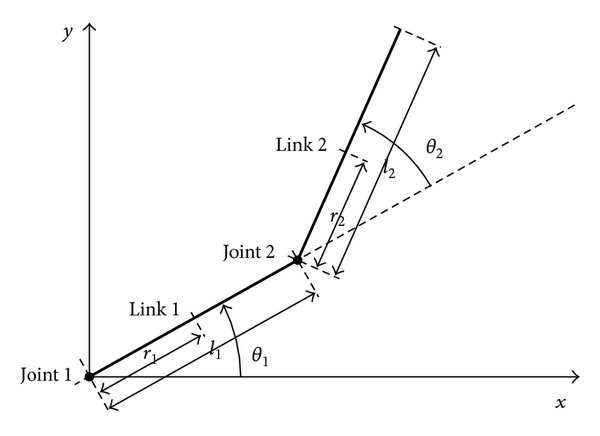
\includegraphics[scale=1.5]{RR.jpg}  
	\caption{Rob\^o \underline{R}\underline{R}}
	\label{fig:figura2}
\end{figure}

	\begin{itemize}
	\item[i)] Primeiro definimos $\nu_q$ coordenadas  $\mq$. Estas podem ser subdivididas em $\nu\ssh$ coordenadas independentes $\mq\ssh$ e $\nu_q^\circ$ 	coordenadas redudantes $\mq^\circ$.
	
	$$
	\mq = \begin{bmatrix}
	\mq\ssh \\
	\mq^\circ
	\end{bmatrix}
	$$

	No caso do mecanismo $\underline{R}\underline{R}$, temos:

	\begin{equation}
	\mq\ssh = \begin{bmatrix}
	\theta_1 & \theta_2
	\end{bmatrix}^T \\
	\end{equation}
	
	\begin{equation}
	\mq^\circ = \begin{bmatrix}
	x_1 & y_1 & x_2 & y_2
	\end{bmatrix}^T
	\end{equation}

	Com $\nu\ssh = 2$ e $\nu_q^\circ = 4$. Neste caso, as componentes de $\mq^\circ$ s\~ao as coordenadas dos centros de massa das barras, escritas no referencial 	inercial $O_{xy}$. \\
	
	\item[ii)] Depois definimos os vetores de velocidades absolutas:
	
	$$ \mw =
	\begin{bmatrix}
	\mw_\omega \\
	\mw_v
	\end{bmatrix}
	$$
	
	\begin{equation}
	\mw_\omega = \begin{bmatrix}
	\omega_{z_1} & \omega_{z_2}
	\end{bmatrix}^T
	\end{equation}
	
	\begin{equation}
	\mw_v = \begin{bmatrix}
	v_{x_1} & v_{y_1} & v_{x_2} & v_{y_2}
	\end{bmatrix}^T
	\end{equation}
	
	Sendo $\mw_v$ as componentes das velocidades absolutas dos centros de massa das barras, escritas nas bases presas às barras, e $\mw_\omega$ as componentes das velocidades angulares absolutas, escritas nas bases presas às barras. \\
	
	\item[iii)] Definimos $\nu_p$ coordenadas  $\mp$. Estas podem ser subdivididas em $\nu\ssh$ coordenadas independentes $\mp\ssh$ e $\nu_p^\circ$ coordenadas redudantes $\mp^\circ$. As coordenadas $\mp\ssh$ podem ser subdividas em $\nu_\omega\ssh$ velocidades angulares $\momega^{\#}$ e $\nu_v\ssh$ velocidades lineares $\mathbb{\nu}\ssh$. As coordenadas $\mp^\circ$ podem ser subdividas em $\nu_\omega^\circ$ velocidades angulares $\momega^\circ$ e $\nu_v^\circ$ velocidades lineares $\mathbb{\nu}^\circ$.
	
	
	\begin{multicols}{3}
	$ \mp = \begin{bmatrix}
	\mp\ssh \\
	\mp^\circ
	\end{bmatrix} $

	$ \mp\ssh = \begin{bmatrix}
	\momega\ssh \\
	\mathbb{\nu}\ssh
	\end{bmatrix} $

	$ \mp^\circ = \begin{bmatrix}
	\momega^\circ \\
	\mathbb{\nu}^\circ
	\end{bmatrix} $

	\end{multicols}
	
	Como \'e conveniente que as velocidades generalizadas $\mp$ sejam velocidades absolutas, escolhemos as componentes de $\mp$ como sendo as mesmas componentes de $\mw$, respeitando a ordena\c{c}\~ao indicada acima. \\ 

	No caso do mecanismo $\underline{R}\underline{R}$, temos:

	\begin{equation}
	\momega\ssh = \begin{bmatrix}
	\omega_{z_1} \\
	\omega_{z_2}
	\end{bmatrix}
	\end{equation}
	
	\begin{equation}
	\mathbb{\nu}\ssh = \emptyset
	\end{equation}		
	
	\begin{equation}
	\momega^\circ = \emptyset
	\end{equation}		
	
	\begin{equation}
	\mathbb{\nu}^\circ = \begin{bmatrix}
	v_{x_1} & v_{y_1} & v_{x_2} & v_{y_2}
	\end{bmatrix}^T
	\end{equation}\\

	Com $\nu_\omega\ssh = 2$, $\nu_v\ssh = 0$, $\nu_\omega^\circ = 0$, $\nu_v^\circ = 4$ e $\nu_p^\circ = \nu_\omega^\circ + \nu_v^\circ = 4$. \\
	
		\item[iv)] Realizamos a cinemática de posi\c{c}\~ao para os centros de massa das barras, de modo a relacionar as coordenadas $\mq^\circ$ com as coordenadas $\mq\ssh$. Para isso, utilizamos matrizes de transforma\c{c}\~ao homog\^enea.



	$$ \nmat{\vH}_{\ttB_0 \rl \ttB_1}  =
	\begin{bmatrix}
	 Rot(\theta_1, z_0) & \nmat{\overrightarrow{\ttO_0 \ttO_1}}_{\ttB_0} \\
	 \mzr_{2x1} & 1 \\
	\end{bmatrix}
	=
	\begin{bmatrix}
	 \ccos_1 & -\ssin_1 & 0 \\
	 \ssin_1 & \ccos_1 & 0 \\
	 0 & 0 & 1 \\
	\end{bmatrix} ;
	\begin{bmatrix}
	\nmat{\overrightarrow{\ttO_1 \ttG_1}}_{\ttB_1} \\
	1
	\end{bmatrix}
	=
	\begin{bmatrix}
	l_{1g} \\
	0 \\
	1 \\
	\end{bmatrix}
	$$

	$$ \nmat{\vH}_{\ttB_1 \rl \ttB_2} =
	\begin{bmatrix}
	 Rot(\theta_2, z_1) & \nmat{\overrightarrow{\ttO_1 \ttO_2}}_{\ttB_1} \\
	 \mzr_{2x1} & 1 \\
	\end{bmatrix}
	=
	\begin{bmatrix}
	 \ccos_2 & -\ssin_2 & l_1 \\
	 \ssin_2 & \ccos_2 & 0 \\
	 0 & 0 & 1 \\
	\end{bmatrix} ;
	\begin{bmatrix}
	 \nmat{\overrightarrow{\ttO_2 \ttG_2}}_{\ttB_2} \\
	1
	\end{bmatrix}
	=
	\begin{bmatrix}
	l_{2g} \\
	0 \\
	1 \\
	\end{bmatrix}
	$$

	$$
	\nmat{\vH}_{\ttB_0 \rl \ttB_2} = \nmat{\vH}_{\ttB_0 \rl \ttB_1} \nmat{\vH}_{\ttB_1 \rl \ttB_2}  =
	\begin{bmatrix}
	\ccos_{1+2} & -\ssin_{1+2} & l_1 \ccos_1 \\
	\ssin_{1+2} & \ccos_{1+2} & l_1 \ssin_1 \\
	0 & 0 & 1 \\
	\end{bmatrix}
	$$


	\begin{equation}
	\therefore \begin{bmatrix}
	x_1 \\
	y_1 \\
	1 \\
	\end{bmatrix}
	=
	\nmat{\vH}_{\ttB_0 \rl \ttB_1}
	\begin{bmatrix}
	\nmat{\overrightarrow{\ttO_1 \ttG_1}}_{\ttB_1} \\
	1
	\end{bmatrix}
	=
	\begin{bmatrix}
	 l_{1g} \ccos_1 \\
	 l_{1g} \ssin_1 \\
	 1 \\
	\end{bmatrix}
	\end{equation}

	\begin{equation}
	\begin{bmatrix}
	x_2 \\
	y_2 \\
	1 \\
	\end{bmatrix}
	=
	\nmat{\vH}_{\ttB_0 \rl \ttB_2}
	\begin{bmatrix}
	 \nmat{\overrightarrow{\ttO_2 \ttG_2}}_{\ttB_2} \\
	1
	\end{bmatrix}
	=
	\begin{bmatrix}
	 l_1 \ccos_1 + l_{2g} \ccos_{1+2} \\
	 l_1 \ssin_1 + l_{2g} \ssin_{1+2} \\
	 1 \\
	\end{bmatrix}
	\end{equation}

	Repare que a partir das matrizes de transforma\c{c}\~ao homogênea encontradas, encontramos também as seguintes matrizes de mudan\c{c}a de base:
	
	\begin{equation}
	\mR_1 = \nmat{\vone}_{\ttB_0 \rl \ttB_1} =
	\begin{bmatrix}
	 \ccos_1 & -\ssin_1  \\
	 \ssin_1 & \ccos_1  \\
	\end{bmatrix}
	\end{equation}
	
	\begin{equation}
	\mR_2 = \nmat{\vone}_{\ttB_0 \rl \ttB_2} =
	\begin{bmatrix}
	 \ccos_{1+2} & -\ssin_{1+2}  \\
	 \ssin_{1+2} & \ccos_{1+2}  \\
	\end{bmatrix}
	\end{equation}		

	Com a cinemática de posi\c{c}\~ao, conseguimos obter $\nu_q^\circ = 4$ equa\c{c}\~oes vinculares de posi\c{c}\~ao. Sendo assim, o vetor dos v\'inculos de posi\c{c}\~ao é dado por:
	
	
	\begin{equation}
	\mphi(\mq)
	=
	\begin{bmatrix}
	x_1 - l_{1g} \ccos_1 \\
	y_1 - l_{1g} \ssin_1 \\
	x_2 - l_1 \ccos_1 - l_{2g} \ccos_{1+2} \\
	y_2 - l_1 \ssin_1 - l_{2g} \ssin_{1+2} \\
	\end{bmatrix}
	\end{equation}
	
	\item[v)] Utilizamos as matrizes de rota\c{c}\~ao para calcular as velocidades angulares em fun\c{c}\~ao de $\mq\ssh$ e $\dot{\mq}\ssh$:
	
	\begin{equation}
	\nsmat{\vomega_1}_{\ttB_1 \rl \ttB_1}  = \mR_1^T \dot{\mR}_1 =
	\begin{bmatrix}
	0 & -\dot{\theta}_1  \\
	\dot{\theta}_1 & 0  \\
	\end{bmatrix}
	\Rightarrow
	\nmat{\vomega_1}_{\ttB_1} = \dot{\theta}_1 \hat{k}
	\end{equation}
	
	\begin{equation}
	\nsmat{\vomega_2}_{\ttB_2 \rl \ttB_2} = \mR_2^T \dot{\mR}_2 =
	\begin{bmatrix}
	0 & -\dot{\theta}_1 -\dot{\theta}_2 \\
	\dot{\theta}_1 + \dot{\theta}_2 & 0  \\
	\end{bmatrix}
	\Rightarrow
	\nmat{\vomega_2}_{\ttB_2} = (\dot{\theta}_1 + \dot{\theta}_2) \hat{k}
	\end{equation}
	
	\item[vi)] Derivamos as equa\c{c}\~oes de posi\c{c}\~ao ((29) e (30)) para encontrar as velocidades dos centros de massa:
	
	\begin{equation}
	\nmat{\vv_1}_{\ttB_0} =
	\begin{bmatrix}
	\dot{x}_1 \\
	\dot{y}_1 \\
	\end{bmatrix}
	=
	\begin{bmatrix}
	- l_{1g} \ssin_1 \dot{\theta}_1 \\
	l_{1g} \ccos_1 \dot{\theta}_1 \\
	\end{bmatrix}
	\end{equation}
	
	\begin{equation}
	\nmat{\vv_2}_{\ttB_0} =
	\begin{bmatrix}
	\dot{x}_2 \\
	\dot{y}_2 \\
	\end{bmatrix}
	=
	\begin{bmatrix}
	- l_1 \ssin_1 \dot{\theta}_1 - l_{2g} \ssin_{1+2} ( \dot{\theta}_1 + \dot{\theta}_2)  \\
	l_1 \ccos_1 \dot{\theta}_1 + l_{2g} \ccos_{1+2} ( \dot{\theta}_1 + \dot{\theta}_2)  \\
	\end{bmatrix}
	\end{equation}
	
	\item[vii)] Passamos as velocidades dos centros de massa para as bases presas nas barras:

	$$ \nmat{\vv_1}_{\ttB_1} = \nmat{\vone}_{\ttB_1 \rl \ttB_0} \nmat{\vv_1}_{\ttB_0} = \mR_1^T \nmat{\vv_1}_{\ttB_0} $$
	$$ \nmat{\vv_2}_{\ttB_2} = \nmat{\vone}_{\ttB_2 \rl \ttB_0} \nmat{\vv_2}_{\ttB_0} = \mR_2^T \nmat{\vv_2}_{\ttB_0} $$
	
	Definindo:
	
	
	\begin{equation}
	\mR_\Diamond =
	\begin{bmatrix}
	\mR_1 & \mzr_{2x2} \\
	\mzr_{2x2} & \mR_2
	\end{bmatrix}
	\end{equation}
	
	Temos:
	
	\begin{equation}
	\mw_v = \mR_\Diamond^T \dot{\mq}^\circ
	\end{equation}
	
	
	\begin{equation}
	\therefore
	\begin{bmatrix}
	v_{x_1} \\
	v_{y_1} \\
	v_{x_2} \\
	v_{y_2} \\
	\end{bmatrix}
	=
	\begin{bmatrix}
	\ccos_1 & -\ssin_1 & 0 & 0 \\
	\ssin_1 & \ccos_1 & 0 & 0 \\
	0 & 0 & \ccos_{1+2} & -\ssin_{1+2} \\
	0 & 0 & \ssin_{1+2} & \ccos_{1+2} \\
	\end{bmatrix}^T
	\begin{bmatrix}
	\dot{x}_1 \\
	\dot{y}_1 \\	
	\dot{x}_2 \\
	\dot{y}_2 \\	
	\end{bmatrix}
	=
	\begin{bmatrix}
	0 \\
	l_{1g} \dot{\theta}_1 \\
	l_1 \ssin_2 \dot{\theta}_1\\
	(l_1 \ccos_2 + l_{2g} )\dot{\theta}_1 + l_{2g} \dot{\theta}_2 \\
	\end{bmatrix}
	\end{equation}
	
	\item[viii)] Montamos os vetores $\mp\ssh$ e $\mp^\circ$ em fun\c{c}\~ao de $\mq\ssh$ e $\dot{\mq}\ssh$:

	\begin{equation}
	\mp\ssh = 
	\begin{bmatrix}
	\omega_{z_1} \\
	\omega_{z_2} \\
	\end{bmatrix}
	= \mp\ssh_\star (\mq\ssh, \dot{\mq}\ssh ) =
	\begin{bmatrix}
	\dot{\theta}_1 \\
	\dot{\theta}_1 +\dot{\theta}_2 \\
	\end{bmatrix}
	\end{equation}
	
	\begin{equation}
	\mp^\circ = 
	\begin{bmatrix}
	v_{x_1} \\
	v_{y_1} \\
	v_{x_2} \\
	v_{y_2} \\
	\end{bmatrix}
	= \mp^\circ_ \star (\mq\ssh, \dot{\mq}\ssh ) =
	\begin{bmatrix}
	0 \\
	l_{1g} \dot{\theta}_1 \\
	l_1 \ssin_2 \dot{\theta}_1\\
	(l_1 \ccos_2 + l_{2g} )\dot{\theta}_1 + l_{2g} \dot{\theta}_2 \\
	\end{bmatrix}
	\end{equation}
	
	\item[ix)] Utilizando o fato de que $\mp\ssh_\star (\mq\ssh, \dot{\mq}\ssh )$ e $\mp^\circ_ \star (\mq\ssh, \dot{\mq}\ssh )$ s\~ao lineares em $\dot{\mq}\ssh$, encontramos as transforma\c{c}\~oes lineares $\mathbb{\Psi}(\mq)$ e $\mathbb{\Upsilon}(\mq)$ e o vetor dos v\'inculos de velocidades $\mathbb{\Lambda}(\mq,\mp)$:
	
	\begin{equation}
	\mp\ssh = \mp\ssh_\star (\mq\ssh, \dot{\mq}\ssh ) = \frac{\partial \mp\ssh_\star}{\partial \dot{\mq}\ssh} \dot{\mq}\ssh = \mathbb{\Psi} \dot{\mq}\ssh
	\end{equation}
	
	\begin{equation}
	\mp^\circ = \mp^\circ_\star (\mq\ssh, \dot{\mq}\ssh ) = \frac{\partial \mp^\circ_\star}{\partial \dot{\mq}\ssh} \dot{\mq}\ssh = \mathbb{\Upsilon} \dot{\mq}\ssh
	\end{equation}

	No caso do mecanismo $\underline{R}\underline{R}$, temos:
	
	\begin{equation}
	\mathbb{\Psi} = \frac{\partial \mp\ssh_\star}{\partial \dot{\mq}\ssh} =
	\begin{bmatrix}
	1 & 0  \\
	1 & 1  \\
	\end{bmatrix}
	\end{equation}
	
	\begin{equation}
	\mathbb{\Upsilon} = \frac{\partial \mp^\circ_\star}{\partial \dot{\mq}\ssh} =
	\begin{bmatrix}
	0 & 0 \\
	l_{1g} & 0 \\
	l_1 \ssin_2 & 0 \\
	l_1 \ccos_2 + l_{2g} & l_{2g} 
	\end{bmatrix}
	\end{equation}\\

	Como $\mp\ssh$ e $\dot{\mq}\ssh$ s\~ao independentes e tem o mesmo tamanho:

	$$ \dot{\mq}\ssh = \mathbb{\Psi}^{-1} \mp\ssh $$
	$$ \Rightarrow  \mp^\circ = \mathbb{\Upsilon} \mathbb{\Psi}^{-1} \mp\ssh $$
	\begin{equation}
	\therefore \mathbb{\Lambda}(\mq,\mp) = \mathbb{\Upsilon} \mathbb{\Psi}^{-1} \mp\ssh - \mp^\circ  = 0
	\end{equation}
	
	\item[x)] A partir dos v\'inculos de velocidades, encontramos a matriz $\mathbb{C}$ dos v\'inculos cinem\'aticos:
	
	$$ \mp^\circ = \mathbb{\Upsilon} \mathbb{\Psi}^{-1} \mp\ssh \Rightarrow \mp =
	\begin{bmatrix}
	\mone\\
	\mathbb{\Upsilon} \mathbb{\Psi}^{-1}
	\end{bmatrix}
	\mp\ssh
	$$
	
	\begin{equation}
	\therefore \mathbb{C} =
	\begin{bmatrix}
	\mone\\
	\mathbb{\Upsilon} \mathbb{\Psi}^{-1}
	\end{bmatrix}
	=
	\begin{bmatrix}
	1 & 0 \\
	0 & 1 \\
	0 & 0 \\
	l_{1g} & 0\\
	l_1 s_{2} & 0 \\
	l_1 c_{2} & l_{2g} \\
	\end{bmatrix}
	\end{equation}
	
	\item[xi)] Como (39) e (43) s\~ao transforma\c{c}\~oes invers\'iveis, encontramos a transforma\c{c}\~ao linear $\mathbb{\Gamma}(\mq)$:
	
	\begin{equation}
	\dot{\mq} =
	\begin{bmatrix}
	\dot{\mq}^{\#} \\
	\dot{\mq}^\circ \\
	\end{bmatrix}
	= \dot{\mq}_\star(\mq,\mp) =
	\begin{bmatrix}
	\mathbb{\Psi}^{-1} (\mq) \mp\ssh \\
	\mR_\Diamond (\mq) \mw_v (\mp)
	\end{bmatrix}
	=
	\begin{bmatrix}
	\omega_{z_1} \\
	\omega_{z_2}-\omega_{z_1}\\
	v_{x_1} \, \ccos_1 - v_{y_1} \, \ssin_1 \\
	v_{x_1} \, \ssin_1 + v_{y_1} \, \ccos_1 \\
	v_{x_2} \, \ccos_{1+2} - v_{y_2} \, \ssin_{1+2} \\
	v_{x_2} \, \ssin_{1+2} + v_{y_2} \, \ccos_{1+2} \\
	\end{bmatrix}
	\end{equation}
	
	\begin{equation}
	\mathbb{\Gamma}(\mq) = \frac{\partial \dot{\mq}_\star}{\partial \mp} =
	\begin{bmatrix}
	1 & 0 & 0 & 0 & 0 & 0 \\
	-1 & 1 & 0 & 0 & 0 & 0 \\
	0 & 0 & \ccos_1 & -\ssin_1 & 0 & 0 \\
	0 & 0 & \ssin_1 & \ccos_1 & 0 & 0 \\
	0 & 0 & 0 & 0 & \ccos_{1+2} & -\ssin_{1+2} \\
	0 & 0 & 0 & 0 & \ssin_{1+2} & \ccos_{1+2} \\
	\end{bmatrix}
	\end{equation}

	\item[xii)] Aplicamos o métodos de Gibbs-Appel extendido: \\
	
	O método de Gibbs-Appell apresenta certa simularidade com o método de Lagrange, pois utiliza derivadas de uma fun\c{c}\~ao energia para encontrar a equa\c{c}\~oes de movimento do sistema. Por\'em, a fun\c{c}\~ao energia utilizada não é a energia cinética, mas sim a energia de acelera\c{c}\~oes. A energia de acelera\c{c}\~oes para um corpo r\'igido \'e dada pela seguinte express\~ao:

	$$ \mathcal{S} = \frac{1}{2} m ( \va_G \cdot \va_G ) + \frac{1}{2}( \dot{\vomega} \cdot \vI \dot{\vomega} + 2 \dot{\vomega} (\vomega \wedge 	\vI \vomega )  )  $$
 
	Sendo $m$ a massa do corpo r\'igido, $\vI$ seu tensor de in\'ercia, $\va_G$ o vetor acelera\c{c}\~ao absoluta de seu centro de massa e $\vomega$ o vetor velocidade angular absoluta.  \\

	O modelo dinâmico utilizando o método de Gibbs-Appel extendido, é dado pela seguinte expressão:
	
	\begin{equation}
	\mC(q)^T ( \mM(\mq) \dot{\mp} + \mv(\mq,\mp) + \mg(\mq)) = (\mathbb{\Psi}^T)^{-1} \mf_{\dot{\mq}\ssh} 
	\end{equation}
	
	Com:
	
	\begin{equation}
	\mM(\mq) = \frac{\partial^2 \mathcal{S}}{\partial \dot{\mp}^2}
	\end{equation}
	
	\begin{equation}
	\mv(\mq,\mp) =  \frac{\partial \mathcal{S}}{\partial \dot{\mp}} - \frac{\partial^2 \mathcal{S}}{\partial \dot{\mp}^2} \dot{\mp}
	\end{equation}
	
	\begin{equation}
	\mg(\mq) =  \mathbb{\Gamma}^T \frac{\partial E_p}{\partial \mq}
	\end{equation}
	
	Sendo $E_p$ a energia potencial do sistema e $\mf_{\dot{\mq}\ssh}$ os esfor\c{c}os nas dire\c{c}\~oes de $\dot{q}^{\#}$. \\
	
	Como j\'a calculamos os vetores de velocidades absolutas dos centros de massa e de velocidades angulares absolutas, escritos em bases presas às barras, as acelera\c{c}\~oes absolutas dos centros de massa são dadas por:
	
	$$ \nvct{\va_i}_{\ttB_i} = \frac{\dd}{\dd t} \nvct{ \vv_i }_{\ttB_i} + \nsmat{\vomega_i}_{\ttB_i \rl \ttB_i}  \nvct{ \vv_i }_{\ttB_i} $$
	
	Como o mecanismo é plano:
	
	$$\nvct{\va_i}_{\ttB_i} = 
	\begin{bmatrix}
	\dot{v}_{x_i} \\
	\dot{v}_{y_i} \\
	\end{bmatrix}
	+
	\begin{bmatrix}
	0  & -\omega_{z_i} \\
	\omega_{z_i} & 0 \\
	\end{bmatrix}
	\begin{bmatrix}
	v_{x_i} \\
	v_{y_i} \\
	\end{bmatrix}
	=
	\begin{bmatrix}
	\dot{v}_{x_i} - \omega_{z_i} v_{y_i} \\
	\dot{v}_{y_i} + \omega_{z_i} v_{x_i}
	\end{bmatrix}
	 $$
	
	No caso do mecanismo $\underline{R}\underline{R}$, temos:
	
	\begin{equation}
	\mathcal{S} = \frac{1}{2} \Big( m_1 ( (\dot{v}_{x_1} - \omega_{z_1} v_{y_1})^2 + (\dot{v}_{y_1} + \omega_{z_1} v_{x_1})^2 ) + m_2 ( (\dot{v}_{x_2} - \omega_{z_2} v_{y_2})^2 + (\dot{v}_{y_2} + \omega_{z_2} v_{x_2})^2  ) + J_{z_1} \dot{\omega}_{z_1}^2 + J_{z_2} \dot{\omega}_{z_2}^2 \Big)
	\end{equation}
	
	\begin{equation}
	E_p = m_1 g y_1 + m_2 g y_2
	\end{equation}
	
	Calculando as derivadas:
	
	\begin{equation}
	\mM(\mq) =
	\begin{bmatrix}
	J_{z_1} & 0 & 0 & 0 & 0 & 0 \\
	0 & J_{z_2} & 0 & 0 & 0 & 0 \\
	0 & 0 & m_1 & 0 & 0 & 0 \\
	0 & 0 & 0 & m_1 & 0 & 0 \\
	0 & 0 & 0 & 0 & m_2 & 0 \\
	0 & 0 & 0 & 0 & 0 & m_2 \\
	\end{bmatrix}
	\end{equation}
	
	\begin{equation}
	\mv(\mq,\mp) =
	\begin{bmatrix}
	0 \\
	0 \\
	-m_1 \omega_{z_1} v_{y_1} \\
	m_1 \omega_{z_1} v_{x_1} \\
	-m_2 \omega_{z_2} v_{y_2} \\
	m_2 \omega_{z_2} v_{x_2} \\
	\end{bmatrix}
	\end{equation}
	
	\begin{equation}
	\mg =
	g \begin{bmatrix}
	0 \\
	0 \\
	m_1  \ssin_1 \\
	m_1  \ccos_1 \\
	m_2  \ssin_{1+2} \\
	m_2  \ccos_{1+2}\\
	\end{bmatrix}
	\end{equation}
	
	Sendo assim, o modelo dinâmico para o mecanismo \underline{R}\underline{R} é dado por:
	
	\begin{equation}
	\begin{bmatrix}
	1 & 0 \\
	0 & 1 \\
	0 & 0 \\
	l_{1g} & 0\\
	l_1 \ssin_{2} & 0 \\
	l_1 \ccos_{2} & l_{2g} \\
	\end{bmatrix}^T
	\begin{Bmatrix}
		\begin{bmatrix}
		J_{z_1} \dot{\omega}_{z_1} \\
		J_{z_2} \dot{\omega}_{z_2} \\
		m_1 \dot{v}_{x_1} \\ 
		m_1 \dot{v}_{y_1} \\
		m_2 \dot{v}_{x_2} \\
		m_2 \dot{v}_{y_2} \\
		\end{bmatrix}
		+
		\begin{bmatrix}
		0 \\
		0 \\
		-m_1 \omega_{z_1} v_{y_1} \\
		m_1 \omega_{z_1} v_{x_1} \\
		-m_2 \omega_{z_2} v_{y_2} \\
		m_2 \omega_{z_2} v_{x_2} \\
		\end{bmatrix}
		+
		g \begin{bmatrix}
		0 \\
		0 \\
		m_1  \ssin_1 \\
		m_1  \ccos_1 \\
		m_1  \ssin_{1+2} \\
		m_1  \ccos_{1+2}\\
		\end{bmatrix}
	\end{Bmatrix}
	=
	\begin{bmatrix}
	1 & 1 \\
	0 & 1 \\
	\end{bmatrix}^{-1}
	\begin{bmatrix}
	\tau_{1} \\
	\tau_{2} \\
	\end{bmatrix}
	\end{equation}
	
	Repare que o modelo não depende das coordenadas $\mq^\circ$. Elas foram uteis para a dedu\c{c}\~ao do modelo, mas com o modelo deduzido elas não tem mais utilidade.
	
	
	
	
	\end{itemize}
\end{itemize}

\begin{itemize}

\item Massa pontual:

\begin{equation}
	\mq_n = \begin{bmatrix}
	x_n \\
	y_n \\
	\end{bmatrix}
	=
	\begin{bmatrix}
	q_{n,1} \\
	q_{n,2} \\
	\end{bmatrix}
\end{equation}

\begin{equation}
	\mp_n = \begin{bmatrix}
	p_{n,1} \\
	p_{n,2} \\
	\end{bmatrix}
	=
	\begin{bmatrix}
	1 & 0 \\
	0 & 1 \\
	\end{bmatrix}
	\begin{bmatrix}
	\dot{q}_{n,1} \\
	\dot{q}_{n,2} \\
	\end{bmatrix}
\end{equation}

\begin{equation}
	\begin{cases}

	\begin{bmatrix}
	\dot{q}_{n,1} \\
	\dot{q}_{n,2} \\
	\end{bmatrix}
	=
	\begin{bmatrix}
	1 & 0 \\
	0 & 1 \\
	\end{bmatrix}
	\begin{bmatrix}
	p_{n,1} \\
	p_{n,2} \\
	\end{bmatrix} \\

	\begin{bmatrix}
	M_n \dot{p}_{n,1} \\
	M_n \dot{p}_{n,2} \\
	\end{bmatrix}
	+
	g \begin{bmatrix}
	0 \\
	M_n \\
	\end{bmatrix}
	=
	\begin{bmatrix}
	f_{n, 1} \\
	f_{n, 2} \\
	\end{bmatrix}
	\end{cases}
\end{equation}

Que pode ser reescrito como:

$$
\begin{bmatrix}
M_n & 0 \\
0 & M_n \\
\end{bmatrix}
\begin{bmatrix}
\ddot{q}_{n,1} \\
\ddot{q}_{n,2} \\
\end{bmatrix}
+
g \begin{bmatrix}
0 \\
M_n \\
\end{bmatrix}
=
\begin{bmatrix}
f_{n,1} \\
f_{n,2} \\
\end{bmatrix}
$$

\item RR:

\begin{equation}
	\mq_n = \begin{bmatrix}
	\theta_{1 \, n} \\
	\theta_{2 \, n} \\
	\end{bmatrix}
	=
	\begin{bmatrix}
	q_{n,1} \\
	q_{n,2} \\
	\end{bmatrix}
\end{equation}

\begin{equation}
	\mp_n = \begin{bmatrix}
	p_{n,1} \\
	p_{n,2} \\
	p_{n,3} \\
	p_{n,4} \\
	p_{n,5} \\
	\end{bmatrix}
	=
	\begin{bmatrix}
	1 & 0 \\
	1 & 1 \\
	l_{g1} & 0\\
	l_1 \ssin_{n,2} & 0 \\
	l_{g2} + l_1 \ccos_{n,2} & l_{g2}
	\end{bmatrix}
	\begin{bmatrix}
	\dot{q}_{n,1} \\
	\dot{q}_{n,2} \\
	\end{bmatrix}
\end{equation}

\begin{equation}
	\begin{cases}

	\begin{bmatrix}
	\dot{q}_{n,1} \\
	\dot{q}_{n,2} \\
	\end{bmatrix}
	=
	\begin{bmatrix}
	1 & 0 \\
	-1 & 1\\
	\end{bmatrix}
	\begin{bmatrix}
	p_{n,1} \\
	p_{n,2} \\
	\end{bmatrix} \\


	\begin{bmatrix}
	1 & 0 \\
	1 & 1 \\
	\end{bmatrix}^T
	\begin{bmatrix}
	 1 & 0 \\
	 0 & 1 \\
	 l_{g1} & 0 \\
	 l_1 \ssin_{n,2} & 0 \\
	 l_1 \ccos_{n,2} & l_{g2} \\
	\end{bmatrix}^T
	\begin{Bmatrix}
		\begin{bmatrix}
		J_{z1} \dot{p}_{n,1} \\
		J_{z2} \dot{p}_{n,2} \\
		m_1 \dot{p}_{n,3} \\
		m_2 \dot{p}_{n,4} \\
		m_2 \dot{p}_{n,5} \\
		\end{bmatrix}
		+
		\begin{bmatrix}
		0 \\
		0 \\
		0 \\
		- m_1 p_{n,2} p_{n,5} \\
		  m_1 p_{n,2} p_{n,4} \\
		\end{bmatrix}
		+
		g \begin{bmatrix}
		0 \\
		0 \\
		m_1 \ccos_{n,1} \\
		m_2 \ssin_{n,1+2} \\
		m_2 \ccos_{n,1+2} \\
		\end{bmatrix}
	\end{Bmatrix}
	=
	\begin{bmatrix}
	u_{n,1} \\
	u_{n,2}
	\end{bmatrix} \\

	\begin{bmatrix}
	l_{g1} & 0 & -1 & 0 & 0 \\
	l_1 \ssin_{n,2} & 0 & 0 & -1 & 0 \\
	l_1 \ccos_{n,2} & l_{g2}  & 0 & 0 & -1 \\
	\end{bmatrix}
	\begin{bmatrix}
	\dot{p}_{n,1} \\
	\dot{p}_{n,2} \\
	\dot{p}_{n,3} \\
	\dot{p}_{n,4} \\
	\dot{p}_{n,5} \\
	\end{bmatrix}
	=
	-
	\begin{bmatrix}
	0 \\
	l_1 \ccos_{n,2} p_{n,1} (-p_{n,1}+p_{n,2}) \\
	l_1 \ssin_{n,2} p_{n,1} (p_{n,1}-p_{n,2}) \\
	\end{bmatrix}

	\end{cases}
\end{equation}

Que pode ser reescrito como:

$$
\begin{bmatrix}
J_{z1} + J_{z2} + m_1 l_{g1}^2 + m_2 (l_1^2 + 2 l_1 l_{g2} \ccos_{n,2} + l_{g2}^2) & J_{z2} + m_2 l_{g2} (l_1 \ccos_{n,2} + l_{g2}) \\
J_{z2} + m_2 l_{g2} (l_1 \ccos_{n,2} + l_{g2}) & J_{z2} + m_2 l_{g2}^2
\end{bmatrix}
\begin{bmatrix}
\ddot{q}_{n,1} \\
\ddot{q}_{n,2} \\
\end{bmatrix}
$$
$$
+
\begin{bmatrix}
- m_2 l_1 l_{g2} \ssin_{n,2} \dot{q}_{n,2}^2 -2 m_2 l_1 l_{g2} \ssin_{n,2} \dot{q}_{n,1}  \dot{q} _{n,2} \\
m_2 l_1 l_{g2} \ssin_{n,2} \dot{q}_{n,1}^2 \\
\end{bmatrix}
+
g \begin{bmatrix}
m_1 l_{g1} \ccos_{n,1} + m_2 (l_{g2} \ccos_{n,1+2} + l_1 \ccos_{n,1}) \\
 m_2 l_{g2} \ccos_{n,1+2} \\
\end{bmatrix}
=
\begin{bmatrix}
u_{n,1} \\
u_{n,2} \\
\end{bmatrix}
$$

\item RR (0) com 2 massas acopladas (1 e 2):

\begin{equation}
	\begin{cases}

	\begin{bmatrix}
	\dot{q}_{0,1} \\
	\dot{q}_{0,2} \\
	\end{bmatrix}
	=
	\begin{bmatrix}
	1 & 0 \\
	-1 & 1\\
	\end{bmatrix}
	\begin{bmatrix}
	p_{0,1} \\
	p_{0,2} \\
	\end{bmatrix} \\

	\begin{bmatrix}
	1 & 0 \\
	1 & 1 \\
	\end{bmatrix}^T
	\begin{bmatrix}
	 1 & 0 \\
	 0 & 1 \\
	 l_{g1} & 0 \\
	 l_1 \ssin_{0,2} & 0 \\
	 l_1 \ccos_{0,2} & l_{g2} \\
	 -L_1 \ssin_{0,1} & 0 \\
	 L_1 \ccos_{0,1} & 0 \\
	 -l_1 \ssin_{0,1} & -L_2 \ssin_{0,1} \\
	 l_1 \ccos_{0,1} & L_2 \ccos_{0,1} \\
	\end{bmatrix}^T
	\begin{Bmatrix}
		\begin{bmatrix}
		J_{z1} \dot{p}_{0,1} \\
		J_{z2} \dot{p}_{0,2} \\
		m_1 \dot{p}_{0,3} \\
		m_2 \dot{p}_{0,4} \\
		m_2 \dot{p}_{0,5} \\
		M_1 \dot{p}_{1,1} \\
		M_1 \dot{p}_{1,2} \\
		M_2 \dot{p}_{2,1} \\
		M_2 \dot{p}_{2,1} \\
		\end{bmatrix}
		+
		\begin{bmatrix}
		0 \\
		0 \\
		0 \\
		- m_1 p_{0,2} p_{0,5} \\
		  m_1 p_{0,2} p_{0,4} \\
		0 \\
		0 \\
		0 \\
		0 \\
		\end{bmatrix}
		+
		g \begin{bmatrix}
		0 \\
		0 \\
		m_1 \ccos_{0,1} \\
		m_2 \ssin_{0,1+2} \\
		m_2 \ccos_{0,1+2} \\
		0 \\
		M_1 \\
		0 \\
		M_2 \\
		\end{bmatrix}
	\end{Bmatrix}
	=
	\begin{bmatrix}
	u_{0,1} \\
	u_{0,2}
	\end{bmatrix} \\

	\begin{bmatrix}
	l_{g1} & 0 & -1 & 0 & 0 & 0 & 0 & 0 & 0 \\
	l_1 \ssin_{i,2} & 0 & 0 & -1 & 0 & 0 & 0 & 0 & 0 \\
	l_1 \ccos_{i,2} & l_{g2}  & 0 & 0 & -1 & 0 & 0 & 0 & 0 \\
	L_1 \ssin_{0,1} & 0 & 0 & 0 & 0 & 1 & 0 & 0 & 0 \\
	-L_1 \ccos_{0,1} & 0 & 0 & 0 & 0 & 0 & 1 & 0 & 0 \\
	l_1 \ssin_{0,1} & L_2 \ssin_{0,1+2}  & 0 & 0 & 0 & 0 & 0 & 1 & 0 \\
	-l_1 \ccos_{0,1} & -L_2 \ccos_{0,1+2} & 0 & 0 & 0 & 0 & 0 & 0 & 1 \\
	\end{bmatrix}
	\begin{bmatrix}
	\dot{p}_{0,1} \\
	\dot{p}_{0,2} \\
	\dot{p}_{0,3} \\
	\dot{p}_{0,4} \\
	\dot{p}_{0,5} \\
	\dot{p}_{1,1} \\
	\dot{p}_{1,2} \\
	\dot{p}_{2,1} \\
	\dot{p}_{2,1} \\
	\end{bmatrix}
	=
	-
	\begin{bmatrix}
	0 \\
	l_1 \ccos_{0,2} p_{0,1} (-p_{0,1}+p_{0,2}) \\
	l_1 \ssin_{0,2} p_{0,1} (p_{0,1}-p_{0,2}) \\
	L_1 \ccos_{0,1} p_{0,1}^2 \\
	L_1 \ssin_{0,1} p_{0,1}^2 \\
	l_1 \ccos_{0,1} p_{0,1}^2 + L_1 \ccos_{0,1+2} p_{0,2}^2  \\
	l_1 \ssin_{0,1} p_{0,1}^2 + L_1 \ssin_{0,1+2} p_{0,2}^2 \\
	\end{bmatrix}

	\end{cases}
\end{equation}

Que pode ser reescrito como:

\begin{equation}
	\mM\ssh \ddot{\mq}_0 + \mv\ssh + \mg\ssh = \mu_0
\end{equation}

Sendo:

\begin{equation}
	\mM\ssh_{1,1} = J_{z1} + J_{z2} + M_1 L_1^2 + M_2 L_2^2 + m_1 l_{g1}^2 + m_2 l_{g2}^2 + (M_2 + m_2)l_1^2 + 2 l_1 \ccos_{0,2} (L_2 M_2 + m_2 l_{g2})
\end{equation}
\begin{equation}
	\mM\ssh_{1,2} = \mM\ssh_{2,1} = J_{z2} + M_2 L_2 (l_1 \ccos_{0,2} + L_2) + m_2 l_{g2} (l_1 \ccos_{0,2} + l_{g2})
\end{equation}
\begin{equation}
	\mM\ssh_{2,2} = J_{z2} + M_2 L_2^2 + m_2 l_{g2}^2
\end{equation}

\begin{equation}
	\mv\ssh_1 = - (M_2 L_2 + m_2 l_{g2}) l_1 \ssin_{0,2} \dot{q}_{0,2} (2 \dot{q}_{0,1} + \dot{q}_{0,2})  
\end{equation}
\begin{equation}
	\mv\ssh_2 = (M_2 L_2 + m_2 l_{g2}) l_1 \ssin_{0,2} \dot{q}_{0,1}^2  
\end{equation}

\begin{equation}
	\mg\ssh_1 = g( M_1 L_1 \ccos_{0,1} + m_1 l_{g1} \ccos_{0,1} + (M_2 + m_2) l_1 \ccos_{0,1} + (M_2 L_2 + m_2 l_{g2}) \ccos_{0,1+2} ) 
\end{equation}

\begin{equation}
	\mg\ssh_2 = g( M_2 L_2 + m_2 l_{g2} ) \ccos_{0,1+2} 
\end{equation}

\item RR balanceado: \\

Escolhendo $L_1$ e $L_2$ de modo que $\mg\ssh = \mzr$:

\begin{equation}
	\begin{cases}
	L_1 = -\frac{ M_2 l_1 + m_1 l_{g1} + m_2 l_2 }{M_1} \\
	L_2 = -\frac{ m_2 l_{g2} }{ M_2 }
	\end{cases}
\end{equation}

Obtemos o seguinte sistema:

\begin{equation}
	\mM\ssh_{1,1} = J_{z1} + J_{z2} + m_1 l_{g2}^2 + l_1^2 (M_2 + m_2) + \frac{m_2^2 l_{g2}^2}{M_2} + \frac{(m_1 l_{g1} + (M_2 + m_2) l_1 )^2 }{M_1}
\end{equation}
\begin{equation}
	\mM\ssh_{1,2} = \mM\ssh_{2,1} = \mM\ssh_{2,2} = J_{z2} + \frac{ m_2 (M_2 + m_2) l_{g2}^2}{M_2}
\end{equation}

\begin{equation}
	\mv\ssh_1 = 0  
\end{equation}
\begin{equation}
	\mv\ssh_2 = 0  
\end{equation}

\begin{equation}
	\mg\ssh_1 = 0
\end{equation}
\begin{equation}
	\mg\ssh_2 = 0
\end{equation}

Ou seja:

\begin{equation}
	\begin{bmatrix}
	J_{z1} + J_{z2} + m_1 l_{g2}^2 + l_1^2 (M_2 + m_2) + \frac{m_2^2 l_{g2}^2}{M_2} + \frac{(m_1 l_{g1} + (M_2 + m_2) l_1 )^2 }{M_1} & J_{z2} + \frac{ m_2 (M_2 + m_2) l_{g2}^2}{M_2} \\
	J_{z2} + \frac{ m_2 (M_2 + m_2) l_{g2}^2}{M_2} & J_{z2} + \frac{ m_2 (M_2 + m_2) l_{g2}^2}{M_2}
	\end{bmatrix}
	\begin{bmatrix}
	\ddot{q}_{n,1} \\
	\ddot{q}_{n,2} \\
	\end{bmatrix}
	=
	\begin{bmatrix}
	u_{n,1} \\
	u_{n,2} \\
	\end{bmatrix}
\end{equation}

\item 5R balanceado: \\

\begin{equation}
	\begin{cases}
	\begin{bmatrix}
	1 & 0 \\
	0 & 1 \\
	\frac{\ccos_{1,1+2}}{l_1 \ssin_{1,2}} &  \frac{\ssin_{1,1+2}}{l_1 \ssin_{1,2}} \\
	-\frac{l_1 \ccos_{1,1} + l_2 \ccos_{1,1+2}}{l_1 l_2 \ssin_{1,2}} &  -\frac{l_1 \ssin_{1,1} + l_2 \ssin_{1,1+2}}{l_1 l_2 \ssin_{1,2}} \\
	\frac{\ccos_{2,1+2}}{l_1 \ssin_{2,2}} &  \frac{\ssin_{2,1+2}}{l_1 \ssin_{2,2}} \\
	-\frac{l_1 \ccos_{2,1} + l_2 \ccos_{2,1+2}}{l_1 l_2 \ssin_{2,2}} &  -\frac{l_1 \ssin_{2,1} + l_2 \ssin_{2,1+2}}{l_1 l_2 \ssin_{2,2}} \\
	\end{bmatrix}^T
	\begin{bmatrix}
	0 & 0 & 0 & 0 & 0 & 0 \\
	0 & 0 & 0 & 0 & 0 & 0 \\
	0 & 0 & \mM\ssh_{1,1} & \mM\ssh_{1,2} & 0 & 0  \\
	0 & 0 & \mM\ssh_{1,2} & \mM\ssh_{1,2} & 0 & 0 \\
	0 & 0 & 0 & 0 & \mM\ssh_{1,1} & \mM\ssh_{1,2}   \\
	0 & 0 & 0 & 0 & \mM\ssh_{1,2} & \mM\ssh_{1,2}  \\
	\end{bmatrix}
	\begin{bmatrix}
	\ddot{q}_{0,1} \\
	\ddot{q}_{0,2} \\
	\ddot{q}_{1,1} \\
	\ddot{q}_{1,2} \\
	\ddot{q}_{2,1} \\
	\ddot{q}_{2,2} \\
	\end{bmatrix}
	=
	\begin{bmatrix}
	\frac{\ccos_{1,1+2}}{l_1 \ssin_{1,2}} &  \frac{\ssin_{1,1+2}}{l_1 \ssin_{1,2}} \\
	\frac{\ccos_{2,1+2}}{l_1 \ssin_{2,2}} &  \frac{\ssin_{2,1+2}}{l_1 \ssin_{2,2}} \\
	\end{bmatrix}
	\begin{bmatrix}
	u_{1,1} \\
	u_{2,1} \\
	\end{bmatrix} \\
	\begin{bmatrix}
	1 & 0 & l_1 \ssin_{1,1} + l_2 \ssin_{1,1+2} & l_2 \ssin_{1,1+2} & 0 & 0 \\
	0 & 1 & -l_1\ccos_{1,1} - l_2 \ccos_{1,1+2} & - l_2 \ccos_{1,1+2} & 0 & 0 \\
	1 & 0 & 0 & 0 & l_1 \ssin_{2,1} + l_2 \ssin_{2,1+2} & l_2 \ssin_{2,1+2}  \\
	0 & 1 & 0 & 0 & -l_1 \ccos_{2,1} - l_2 \ccos_{2,1+2} & - l_2 \ccos_{2,1+2} \\
	\end{bmatrix}
	\begin{bmatrix}
	\ddot{q}_{0,1} \\
	\ddot{q}_{0,2} \\
	\ddot{q}_{1,1} \\
	\ddot{q}_{1,2} \\
	\ddot{q}_{2,1} \\
	\ddot{q}_{2,2} \\
	\end{bmatrix}
	= \\
	- \begin{bmatrix}
	l_1 \ccos_{1,1} \dot{q}_{1,1}^2 + l_2 \ccos_{1,1+2} (\dot{q}_{1,1}+\dot{q}_{1,2})^2 \\
	l_1 \ssin_{1,1} \dot{q}_{1,1}^2 + l_2 \ssin_{1,1+2} (\dot{q}_{1,1}+\dot{q}_{1,2})^2 \\
	l_1 \ccos_{2,1} \dot{q}_{2,1}^2 + l_2 \ccos_{2,1+2} (\dot{q}_{2,1}+\dot{q}_{2,2})^2 \\
	l_1 \ssin_{2,1} \dot{q}_{2,1}^2 + l_2 \ssin_{2,1+2} (\dot{q}_{2,1}+\dot{q}_{2,2})^2 \\
	\end{bmatrix}
	\end{cases}
\end{equation}

\end{itemize}

%\subsection{Introduction to sliding modes control}\label{S02-3}

In this subsection, a brief introduction to the sliding modes control will be done. The theme will be explored only to perform second order systems control, without parametric uncertainties, to not escape the scope of the chapter. \\

Consider a dynamical system given by the following differential equation:
\begin{equation} \label{eq:SimpleODE}
\ddot{x} = u
\end{equation}

A curve in the error phase plan, called sliding surface, can be defined:
\begin{equation} \label{eq:SlidingSurface}
s(e, \dot{e}) = - (\dot{e} + \lambda e) = 0, \, \lambda > 0
\end{equation}

Being $e = x^\sdia - x$ the error signal and $x^\diamond$ reference signal. Note that if the system is on the sliding surface, we have:
\begin{equation} \label{eq:SlidingError}
\dot{e} + \lambda e = 0 \Rightarrow e(t) = c \, \mathsf{e}^{- \lambda t}
\end{equation}

Thus, the error drops exponentially to zero, with time constant $1/\lambda$.

To find a control law that brings the system to the sliding surface, we start from the definition of $s$: \\

$ s = -(\dot{e} + \lambda e) $ \\

Differentiating with respect to time:

\begin{equation} \label{eq:dotS}
\dot{s} =  -(\ddot{e} + \lambda \dot{e}) = \ddot{x} - \ddot{x}^\sdia - \lambda \dot{e} 
\end{equation}

Substituting \eqref{eq:SimpleODE} into \eqref{eq:dotS}:
\begin{equation} \label{dotS2}
\dot{s} = u - \ddot{x}^\sdia - \lambda \dot{e}
\end{equation}

Using the following control law:
\begin{equation} \label{SMControlLaw1D}
u = \ddot{x}^\sdia + \lambda \dot{e} - k \sign (s), \, k>0
\end{equation}

He have:
\begin{equation} \label{CloserLoop1D}
\dot{s} = -k \sign(s) 
\end{equation}

Suppose that the system starts at $s(0) = s_0 >0$. Solving the ODE for $s>0$:

$$ \dot{s} = -k \Rightarrow s = -k t + c $$
$$ s(0) = s_0 \Rightarrow c = s_0 $$
$$ \therefore s = s_0 - k t, \, s>0 $$

According to the solution found, when $t \rightarrow t_s = \frac{|s_0|}{k}$, $s \rightarrow 0 $. Solving the ODE for $s(t_s) = 0$:

$$ \dot{s} = 0 \Rightarrow s =  c $$
$$ s(t_s) = 0 \Rightarrow c = 0 $$

Therefore, the solution of the ODE for $s(0) = s_0 > 0$ is given by:
\begin{equation} \label{eq:SM-ODE-Sol1}
s(t) =
\begin{cases}
s_0 - k t, \, t < t_s \\
0, \,\,\,\,\,\,\,\,\,\,\,\,\,\,\,\, t \geq t_s \\
\end{cases}
\end{equation}

An analogous result is found solving the ODE for $s(0) = s_0 < 0$:

\begin{equation} \label{eq:SM-ODE-Sol2}
s(t) =
\begin{cases}
s_0 + k t, \, t < t_s \\
0, \,\,\,\,\,\,\,\,\,\,\,\,\,\,\,\, t \geq t_s \\
\end{cases}
\end{equation}

Thus, it can be concluded that the ODE \eqref{CloserLoop1D} converges to $s=0$, regardless of the initial condition.
Therefore, we have that the control law \eqref{SMControlLaw1D} makes the system represented by \eqref{eq:SimpleODE} follow the reference signal, because the error signal converges to zero.



%\subsection{Extended sliding modes control techniques}\label{S02-4}

As seen in subsections 2.1 and 2.2, it's very convenient to use redundant coordinates to perform parallel mechanism dynamic modeling. 
The aim of this subsection it to propose a control law for systems described by redundant coordinates.

Let $\ssM$ be a multibody mechanical system whose mathematical model is given 
by equations~(\ref{eq:02-105B},~\ref{eq:02-112B}).
For the sake of brevity, no system index $n$ will be used in this subsection.
Suppose that each $\mf$ is an affine function of the control inputs $u_{k}$
in which the coefficients of the $u_{k}$ may depend on the instantaneous
configuration of the system.
Suppose additionally that that all the $\mA$ are independent
of the quasi-velocities $p_{j}$ and all the $\mM$, $\mg$, $\mA$ and $\mb$ 
are independent of the $u_{k}$.
Under these conditions, matrices $\mC$ will not depend on 
any quasi-velocity, $\md$ can be expressed as an affine function of the control inputs 
and $\mc$ is independent of them.
Considering that the number of control inputs in $\ssM$ is
exactly equal to the number of degrees of freedom of $\ssM$, 
there exists a particular matrix $\mC(t,\mq)$ such that:
\begin{equation} \label{eq:InverseDynamics}
\mu = \mC^\msT(t,\mq) \Big( \mM (t, \mq) \, \dot{\mp} + \mw(t,\mq,\mp) + \mz(t,\mq) \Big)
\end{equation}
In equation \eqref{eq:InverseDynamics}, $\mw$ is a column-vector representing terms of generalized force 
or generalized gyroscopic inertia force which are linear or bilinear with respect to quasi-velocities 
and $\mz$ stems from terms that are independent of these variables.

From the control perspective, it is convenient to work with mathematical models in which $\mp = \dot \mq$, 
in order to have a position feedback control.
Thus, based on equations \eqref{eq:InverseDynamics} and \eqref{eq:02-201A}, consider that 
the mathematical model of $\ssM$ is given by the following equations:
\begin{equation} \label{eq:MechanicalSystem}
\begin{cases}
\mC^\msT (t, \mq) \Big( \mM (t, \mq) \, \ddot{\mq} + \mw (t, \mq, \dot{\mq}) + \mz (t, \mq) \Big) = \mu \\
\mA (t, \mq) \, \ddot{\mq} + \mb (t, \mq, \dot{\mq}) = \mzr
\end{cases}
\end{equation}
Rewriting in a compact matrix form:
\begin{equation} \label{eq:MechanicalSystemMatrix}
\begin{bmatrix}
\mC^\msT \mM \\
\mA
\end{bmatrix}
\ddot{\mq}
=
\begin{bmatrix}
\mu - \mC^\msT(\mw + \mz) \\
-\mb
\end{bmatrix}
\end{equation}
The desired control law should satisfy, in closed loop, the condition $ \ddot{\mq} = \mv $, with $\mv$ being 
a control input column-matrix. 
Thus, the following control law should be used:
\begin{equation} \label{eq:ControlLawV}
\mu = \mC^\msT ( \mM \, \mv + \mw + \mz )
\end{equation}
Once $ \ddot{\mq} = \mv $, and $\ddot{\mq}$ has to satisfy constraint equations, $\mv$ must respect the same restrictions, i.e.:
\begin{equation} \label{eq:ControlLawVRestriction}
\mA \, \mv + \mb = \mzr
\end{equation}
Applying the control law \eqref{eq:ControlLawV} and the 
rectritions \eqref{eq:ControlLawVRestriction} in \eqref{eq:MechanicalSystemMatrix}: 
\begin{align*}
&	\begin{bmatrix}
	\mC^\msT \, \mM \\
	\mA
	\end{bmatrix}
	\ddot{\mq}
	=
	\begin{bmatrix}
	\mC^\msT ( \mM \, \mv + \mw + \mz ) - \mC^\msT(\mw + \mz) \\
	\mA \, \mv
	\end{bmatrix}
	=
	\begin{bmatrix}
	\mC^\msT  \, \mM \, \mv \\
	\mA \, \mv
	\end{bmatrix}
	=
	\begin{bmatrix}
	\mC^\msT \mM \\
	\mA
	\end{bmatrix}
	\mv 
\end{align*}
Once the matrix $\begin{bmatrix} \mC^\msT \, \mM \\ \mA \end{bmatrix}$ is non-singular:
\begin{equation} \label{eq:ClosedLoopV}
\ddot{\mq} = \mv
\end{equation}

Let $\mv'$ be given by the sliding modes control law:
\begin{equation} \label{eq:SMControlowLasV1'}
\mv' = \ddot{\mq}^\sdia + \lambda \dot{\me} + k \sign (\dot{\me} + \lambda \me)
\end{equation}
Being $ \me = \mq^\sdia - \mq $ the error signal and $\mq^\sdia$ the reference signal. If there were no retrictions, it could be stated that $ \mv = \mv' $, and:
\begin{align*}
	\ddot{\mq} = \mv \qquad \Rightarrow \qquad \ddot{\me} + \lambda \dot{\me} + k \sign (\dot{\me} + \lambda \me) = \mzr 
	\qquad \Leftrightarrow \qquad \dot{\ms} = - k \sign(\ms)
\end{align*}
This would ensure that $\me \rightarrow 0$ when $t \rightarrow \infty$ for any initial condition, as seen in the last subsection. 

Once $\mv$ can not be freely set as $\mv'$, the following optimization problem is proposed:
\begin{align} \label{eq:Optimization}
& 	\min_{\mv} \quad (\mv - \mv')^\msT \, \mM \, (\mv - \mv') 
	\qquad \text{s.t.} \qquad \mA \, \mv + \mb = \mzr
\end{align}
As $\mM$ is positive-semidefinite, then $(\mv - \mv')^\msT \, \mM \, (\mv - \mv') \geq 0 $ for any $\mv$.

Applying the method of Lagrange undetermined multipliers, it can be stated that this
optimization problem is equivalent to minimize with respect to $\mv$ and $\mlambda$
the following functional:
\begin{equation}
L = (\mv - \mv')^\msT \, \mM \, (\mv - \mv') + (\mA \mv + \mb)^\msT \, \mlambda 
\end{equation}
To solve the problem, the Lagrangian function must be stationary. Thus:
\begin{align}
 	\dl L = 0 \qquad &\Rightarrow \qquad  
 	\dl \mv^\msT \mM (\mv - \mv') + (\mv - \mv')^\msT \mM \dl \mv + (\mA \dl \mv)^\msT \mlambda 
		+ (\mA \mv + \mb)^\msT \dl \mlambda = 0 
	\nonumber \\	
& 	\Rightarrow \qquad
	\dl \mv^\msT \left( (\mM + \mM^\msT)(\mv - \mv') + \mA^\msT \mlambda \right) + \dl \mlambda^\msT (\mA \mv + \mb) = 0 
\end{align}
Once $\mM$ is symmetric and $\dl \mv$ and $\dl \mlambda$ are arbitrary:
\begin{equation} \label{eq:OptimizationSol}
\begin{cases}
2 \, \mM \, (\mv - \mv') + \mA^\msT \mlambda = \mzr \\
\mA \, \mv + \mb = \mzr
\end{cases}
\end{equation}
Considering that $\mC$ is an orthogonal complement of $\mA$, pre-multiplying the first equation of 
\eqref{eq:OptimizationSol} by $\mC^\msT$ leads to:
\begin{align}
& 	2 \, \mC^\msT \, \mM (\mv - \mv') + \mC^\msT \, \mA^\msT \mlambda = \mzr 
	\qquad 	\Rightarrow \qquad \mC^\msT \, \mM (\mv - \mv')  = \mzr 
	\qquad \therefore \qquad \mC^\msT \, \mM \, \mv  = \mC^\msT \, \mM \, \mv'
	\label{eq:OptimizationSol2}
\end{align}
Thus, the control law that makes the closed loop system as close as possible of $\ddot{\mq} = \mv'$, 
according to the optimization criterion adopted, is:
\begin{equation} \label{eq:ControlLawFinal}
\mu = \mC^\msT ( \mM \, \mv' + \mw + \mz )
\end{equation}

\begin{figure}[H]
	\centering
	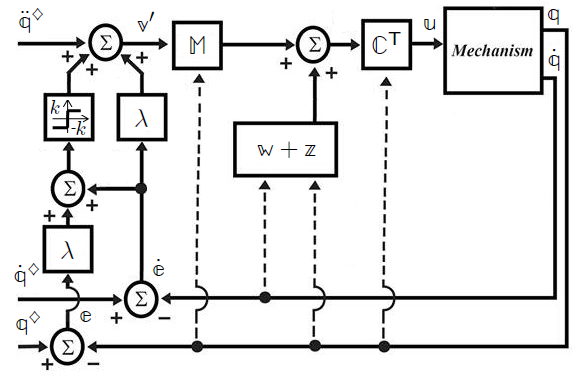
\includegraphics[scale=0.75]{ControlDiagram.png}
	\caption{Control block diagram}
	\label{ControlDiagram}
\end{figure}




%--------------------BALANCING--------------------%

%\input{SECTIONS/RENATO/3-1}

%\subsection{Control}\label{S03-2}
 
\noindent {\bf Controle por modos deslizantes}\\

Nesta se\c{c}\~ao ser\'a feita uma breve introdu\c{c}\~ao ao controle por modos deslizantes. O tema ser\'a explorado apenas para o controle de sistemas de segunda ordem, sem incertezas param\'etricas, para n\~ao fugir do escopo do cap\'itulo. \\

Seja um sistema din\^amico dado pela seguinte equa\c{c}\~ao diferencial:
\begin{equation} \label{eq:SimpleODE}
\ddot{x} = u
\end{equation}

Definimos a seguinte superf\'icie, chamada de superf\'icie de escorregamento:
\begin{equation} \label{eq:SlidingSurface}
s(e, \dot{e}) = - (\dot{e} + \lambda e) = 0, \, \lambda > 0
\end{equation}

Sendo $e = x_d - x$ o erro de controle e $x_d$ o sinal de refer\^encia. Repare que se o sistema estiver na superf\'icie de escorregamento, temos:
\begin{equation} \label{eq:SlidingError}
\dot{e} + \lambda e = 0 \Rightarrow e(t) = C e^{- \lambda t}
\end{equation}

Sendo assim, o erro cai exponencialmente para zero, com constante de tempo $1/\lambda$.

Para encontrar a lei de controle que leva o sistema \`a superf\'icie de escorregamento, parte-se da defini\c{c}\~ao de $s$:

$$ s = -(\dot{e} + \lambda e) $$

Derivando no tempo:
\begin{equation} \label{eq:dotS}
\dot{s} =  -(\ddot{e} + \lambda \dot{e}) = \ddot{x} - \ddot{x}_d - \lambda \dot{e} 
\end{equation}

Substituindo \eqref{eq:SimpleODE} em \eqref{eq:dotS}:
\begin{equation} \label{dotS2}
\dot{s} = u - \ddot{x}_d - \lambda \dot{e}
\end{equation}

Utizando a seguinte lei de controle:
\begin{equation} \label{SMControlLaw1D}
u = \ddot{x}_d + \lambda \dot{e} - k \sign (s), \, k>0
\end{equation}

Temos:
\begin{equation} \label{CloserLoop1D}
\dot{s} = -k \sign(s) 
\end{equation}

Supondo que o sistema come\c{c}a em $s(0) = s_0 >0$. Resolvendo a EDO para $s>0$:

$$ \dot{s} = -k \Rightarrow s = -k t + C $$
$$ s(0) = s_0 \Rightarrow C = s_0 $$
$$ \therefore s = s_0 - k t, \, s>0 $$

Em $t = t_s = \frac{|s_0|}{k}$, $s$ chega em zero. Resolvendo a EDO para $s(t_s) = 0$:

$$ \dot{s} = 0 \Rightarrow s =  C $$
$$ s(t_s) = 0 \Rightarrow C = 0 $$

Portanto, para a solu\c{c}\~ao da EDO para $s(0) = s_0 > 0$ é
\begin{equation} \label{eq:SM-ODE-Sol1}
s(t) =
\begin{cases}
s_0 - k t, \, t < t_s \\
0, \,\,\,\,\,\,\,\,\,\,\,\,\,\,\,\, t \geq t_s \\
\end{cases}
\end{equation}

Resolvendo para $s(0) = s_0 < 0$, temos um resultado an\'alogo:

\begin{equation} \label{eq:SM-ODE-Sol2}
s(t) =
\begin{cases}
s_0 + k t, \, t < t_s \\
0, \,\,\,\,\,\,\,\,\,\,\,\,\,\,\,\, t \geq t_s \\
\end{cases}
\end{equation}

Assim, pode-se concluir que a EDO \eqref{CloserLoop1D} converge para $s=0$, independente da condi\c{c}\~ao inicial. Portanto, temos que a lei de controle \eqref{SMControlLaw1D} faz o sistema \eqref{eq:SimpleODE} siga o sinal de referência, pois o erro de controle converge para zero. \\

\noindent {\bf Controle por modos deslizantes extendido}\\

Como foi visto na seção de modelagem, é muito conveniente utilizar coordenadas redundantes para realizar a modelagem de mecanismos paralelos. Sendo assim, propomos nesta seção uma lei de controle para sistemas descritos com coordenadas redundantes. \\
 
O modelo de um sistema mec\^anico multi-corpos pode ser descrito de maneira gen\'erica pelas seguintes equa\c{c}\~oes:
\begin{equation} \label{eq:MechanicalSystem}
\begin{cases}
\mC_n^\top (\mq_n) \Big( \mM_n (\mq_n) \ddot{\mq}_n + \mw_n (\mq_n, \dot{\mq}_n) + \mz_n (\mq_n) \Big) = \mu_n \\
\mA_n \ddot{\mq}_n + \mb_n (\mq_n, \dot{\mq}_n) = \mzr
\end{cases}
\end{equation}

De maneira matricial compacta:
\begin{equation} \label{eq:MechanicalSystemMatrix}
\begin{bmatrix}
\mC_n^\top \mM_n \\
\mA_n
\end{bmatrix}
\ddot{\mq}_n
=
\begin{bmatrix}
\mu_n - \mC_n^\top(\mw_n + \mz_n) \\
-\mb_n
\end{bmatrix}
\end{equation}

Gostaria que $ \ddot{\mq}_n = \mv_n $, sendo $\mv_n$ uma entrada de controle. Para que isso aconte\c{c}a, utilizamos a seguinte lei de controle:
\begin{equation} \label{eq:ControlLawV}
\mu_n = \mC_n^\top ( \mM_n \mv_n + \mw_n + \mz_n )
\end{equation}

Como queremos que $ \ddot{\mq}_n = \mv_n $ e $\ddot{\mq}_n$ tem restri\c{c}\~oes, $\mv_n$ deve respeitar as mesmas restri\c{c}\~oes, ou seja:
\begin{equation} \label{eq:ControlLawVRestriction}
\mA_n \mv_n + \mb_n = \mzr
\end{equation}

Aplicando a lei de controle \eqref{eq:ControlLawV} em \eqref{eq:MechanicalSystemMatrix}, temos:
\begin{center}
$ \begin{bmatrix}
\mC_n^\top \mM_n \\
\mA_n
\end{bmatrix}
\ddot{\mq}_n
=
\begin{bmatrix}
\mC_n^\top ( \mM_n \mv_n + \mw_n + \mz_n ) - \mC_n^\top(\mw_n + \mz_n) \\
\mA_n \mv_n
\end{bmatrix}
=
\begin{bmatrix}
\mC_n^\top  \mM_n \mv_n \\
\mA_n \mv_n
\end{bmatrix}
=
\begin{bmatrix}
\mC_n^\top \mM_n \\
\mA_n
\end{bmatrix}
\mv_n $
\end{center}
\begin{equation} \label{eq:ClosedLoopV}
\therefore \ddot{\mq}_n = \mv_n
\end{equation}

Seja $\mv'_n$ dado pela lei de controle por modos deslizantes:
\begin{equation} \label{eq:SMControlowLasV1'}
\mv'_n = \ddot{\mq}_{n, d} + \lambda \dot{\me}_n + k \sign (\dot{\me}_n + \lambda \me_n)
\end{equation}
Sendo $ \me_n = \mq_{n,d} - \mq_n $ o erro de controle de $\mq_{n,d}$ o sinal de ref\^encia. Se n\~ao houvesse restri\c{c}\~oes, poderiamos fazer $ \mv_n = \mv'_n $ :
$$ \ddot{\mq}_n = \mv_n \Rightarrow  \ddot{\me}_n + \lambda \dot{\me}_n + k \sign (\dot{\me}_n + \lambda \me_n) = \mzr$$
Isso garantiria que $\me_n \rightarrow 0$ quando $t \rightarrow \infty$ para quaisquer condi\c{c}\~oes iniciais. \\

Como temos restri\c{c}\~oes em $\mv_n$, procuramos $\mv_n$ mais pr\'oximo poss\'ivel de $\mv'_n$ atraves da solu\c{c}\~ao do seguinte problema de otimiza\c{c}\~ao:

\begin{center}
$\begin{aligned}
& \underset{\mv_n}{\text{Min}}
& & (\mv_n - \mv'_n)^\top \mM_n (\mv_n - \mv'_n) \\
& \text{tal que}
& & \mA_n \mv_n + \mb_n = \mzr
\end{aligned}$
\end{center}

Como $\mM_n$ \'e n\~ao-negativa definida, temos que $(\mv_n - \mv'_n)^\top \mM_n (\mv_n - \mv'_n) \geq 0 $ para qualquer valor de $\mv_n$.

Aplicando a t\'enica dos multiplicadores de Lagrange, pode-se dizer que o seguinte problema é equivalente:

\begin{center}
$\begin{aligned}
& \underset{\mv_n, \mlambda}{\text{Min}}
& & \llL = (\mv_n - \mv'_n)^\top \mM_n (\mv_n - \mv'_n) + (\mA_n \mv_n + \mb_n)^\top \mlambda \\
\end{aligned}$
\end{center}

Para solucionar o problema, imp\~oe-se a estacionariedade da fun\c{c}\~ao lagrangeana:

$$ \dl \llL = 0 \Rightarrow \dl \mv_n^\top \mM_n (\mv_n - \mv'_n) + (\mv_n - \mv'_n)^\top \mM_n \dl \mv_n + (\mA_n \dl \mv_n)^\top \mlambda + (\mA_n \mv_n + \mb_n)^\top \dl \mlambda = 0 $$
$$ \Rightarrow \dl \mv_n^\top \Big( (\mM_n + \mM_n^\top)(\mv_n - \mv'_n) + \mA_n^\top \mlambda \Big) + \dl \mlambda^\top (\mA_n \mv_n + \mb_n) = 0 $$

Como $\mM_n$ é sim\'etrica e $\dl \mv_n$ e $\dl \mlambda$ são arbitr\'arios, temos:

$$
\begin{cases}
2 \mM_n (\mv_n - \mv'_n) + \mA_n^\top \mlambda = \mzr \\
\mA_n \mv_n + \mb_n = \mzr
\end{cases}
$$

Como $\mC_n$ é o complemento ortogonal de $\mA_n$, multiplicando a primeira equa\c{c}\~ao por $\mC_n^\top$, temos:

$$ 2 \mC_n^\top \mM_n (\mv_n - \mv'_n) + \mC_n^\top \mA_n^\top \mlambda = \mzr $$
$$ \Rightarrow  \mC_n^\top \mM_n (\mv_n - \mv'_n)  = \mzr $$
$$ \therefore \mC_n^\top \mM_n \mv_n  = \mC_n^\top \mM_n  \mv'_n $$

Sendo assim, temos que a lei de controle que torna o sistema em malha fechado o mais pr\'oximo poss\'ivel, segundo o crit\'erio de otimiza\c{c}\~ao adotado, de $\ddot{\mq}_n = \mv'$ \'e:

$$ \mu_n = \mC_n^\top ( \mM_n \mv'_n + \mw_n + \mz_n ) $$

\newpage



$$
\begin{bmatrix}
\mC^T \mM \\
\mA
\end{bmatrix}
\ddot{\mq}
=
\begin{bmatrix}
\mathbb{\zeta} \mu \\
-\mb
\end{bmatrix}
$$



$$ \mu = \mathbb{\zeta}^{-1} \mC^T \mM \mu' $$
$$ \mu' = \ddot{\mq}_d + \lambda \dot{\me} - k  \sign (\ms) $$

$$ \ms = - \dot{\me} - \lambda \me $$
$$ \dot{\ms} = - \ddot{\me} - \lambda \dot{\me} = \ddot{\mq} - \ddot{\mq}_d  - \lambda \dot{\me} $$
$$ \dot{\ms} =  \begin{bmatrix}
\mC^T \mM \\
\mA
\end{bmatrix}^{-1}
\begin{bmatrix}
\mathbb{\zeta} \mu \\
-\mb
\end{bmatrix}
 - \ddot{\mq}_d  - \lambda \dot{\me} $$
 
Aplicando a lei de controle:

$$ \dot{\ms} =  \begin{bmatrix}
\mC^T \mM \\
\mA
\end{bmatrix}^{-1}
\begin{bmatrix}
 \mC^T \mM (\ddot{\mq}_d + \lambda \dot{\me} - k  \sign (\ms)) \\
-\mb
\end{bmatrix}
 - \ddot{\mq}_d  - \lambda \dot{\me} $$
 
 $$ \dot{\ms} =  \begin{bmatrix}
\mC^T \mM \\
\mA
\end{bmatrix}^{-1}
\begin{bmatrix}
 \mC^T \mM (\ddot{\mq}_d + \lambda \dot{\me} - k  \sign (\ms)) -  \mC^T \mM(\ddot{\mq}_d  + \lambda \dot{\me}) \\
-\mb - \mA(\ddot{\mq}_d  + \lambda \dot{\me})
\end{bmatrix} $$

 $$ \dot{\ms} =  \begin{bmatrix}
\mC^T \mM \\
\mA
\end{bmatrix}^{-1}
\begin{bmatrix}
- \mC^T \mM  k  \sign (\ms) \\
-\mb - \mA(\ddot{\mq}_d  + \lambda \dot{\me})
\end{bmatrix} $$

Definindo:
$$\begin{bmatrix}
\mC^T \mM \\
\mA
\end{bmatrix}^{-1}
=
\begin{bmatrix}
(\mC^T \mM)^\dagger & \mA^\dagger
\end{bmatrix} $$

Temos:

$$\dot{\ms} = 
- (\mC^T \mM)^\dagger \mC^T \mM  k  \sign (\ms) - \mA^\dagger\mb - \mA^\dagger \mA(\ddot{\mq}_d  + \lambda \dot{\me}) $$

Sendo assim, se a seguinte inequação for respeitada para pelo menos $\nu\ssh$ componentes de $\dot{\ms}$, o erro vai a zero:

$$\dot{\ms} = 
- (\mC^T \mM)^\dagger \mC^T \mM  k  \sign (\ms) - \mA^\dagger\mb - \mA^\dagger \mA(\ddot{\mq}_d  + \lambda \dot{\me}) \leq \mzr $$


%--------------------EXAMPLE---------------------%

%% \section{Ex}\label{S04}

% \subsection{5R}\label{S04-1}

%% \subsection{Delta}\label{S04-2}

%\input{SECTIONS/RENATO/4-3}

\subsection{Inverse Dynamics and Control Simulations}\label{S04-4}

Dada a lei de controle apresentada na sub-se\c{c}\~ao 2.4 e o modelo din\^amico apresentado na sub-se\c{c}\~ao anterior, nesta sub-se\c{c}\~ao realizaremos simula\c{c}\~oes da din\^amica inversa e da aplica\c{c}\~ao da lei de controle nos modelos $\mathru{RR{\ud}G}$ e $\mathru{RR{\ud}U}$. Para tanto, \'e necess\'ario definir valores para os par\^ametros do mecanismos, as condi\c{c}\~oes iniciais do sistema, trajetórias de referência e os par\^ametros do controlador.

Assim, definimos:

\begin{itemize}
\item Par\^ametros f\'isicos fixos dos modelos RR\ud utilizados para formar o modelo 5R\ud:

\begin{itemize}
\begin{multicols}{2}
\item[\bf \----] $a_{1,1} = 0.1 \, m$
\item[\bf \----] $a_{1,2} = 0.2 \, m$
\item[\bf \----] $m_{1, \llB_1} = 0.2 \, kg$
\item[\bf \----] $m_{1, \llB_2} = 0.4 \, kg$
\item[\bf \----] $m_{2, \llB_1} = 1.5 \, kg$
\item[\bf \----] $I_{1, \llB_1} = 67 \cdot 10^{-5} \, kg \, m^2$
\item[\bf \----] $I_{1, \llB_2} = 134 \cdot 10^{-5} \, kg \, m^2$
\item[\bf \----] $\gamma_{1, \llB_1} = \gamma_{1, \llB_2} = 0.5$
\end{multicols}
\end{itemize}

\item Par\^ametros físicos ajustáveis do modelo $\mathru{RR{\ud}G}$:

\begin{itemize}
\begin{multicols}{2}
\item[\bf \----] $\gamma_{3, \llB_1} = 3.0$
\item[\bf \----] $\gamma_{4, \llB_1} = 1.7$
\item[\bf \----] $m_{3, \llB_1} = m_{4, \llB_1} = 1.0 \, kg$ 
\end{multicols}
\end{itemize}

\item Par\^ametros físicos ajustáveis do modelo $\mathru{RR{\ud}U}$:

\begin{itemize}
\item[\bf \----] $m_{3, \llB_1} = m_{4, \llB_1} = 0$
\end{itemize}


\item Posicionamento das bases dos modelos RR\ud para formar o modelo 5R\ud:

\begin{itemize}
\begin{multicols}{2}
\item[\bf \----] $q_{1,\ttp_1,1} = -0.1 \, m$
\item[\bf \----] $q_{1,\ttp_1,2} = 0 $
\item[\bf \----] $q_{2,\ttp_1,1} = 0.1 \, m$
\item[\bf \----] $q_{2,\ttp_1,2} = 0 $
\end{multicols}
\end{itemize}

\item Par\^ametros do controlador utilizado:

\begin{itemize}
\begin{multicols}{2}
\item[\bf \----] $\lambda = 40$
\item[\bf \----] $k = 10$
\end{multicols}
\end{itemize}

\item Condi\c{c}\~oes iniciais de posi\c{c}\~ao para o modelo 5R\ud:

$$\begin{cases}
q_{1,\ttp_3,1}(0) = q_{2,\ttp_3,1}(0) = 0 \\
q_{1,\ttp_3,2}(0) = q_{2,\ttp_3,2}(0) = 0.02 \,m \\
q_{3, \llR_3}(0) = 173.282^\circ \\
q_{1,\llR_1}(0) = 175.249^\circ \\
q_{1,\llR_2}(0) = 188.11^\circ \\
q_{2,\llR_1}(0) = 4.75078^\circ \\
q_{2,\llR_2}(0) = 171.89^\circ \\
\end{cases}$$

\item Trajet\'oria de refer\^encia 1:

$$ \begin{cases}
q_{1,\ttp_3,1}^\sdia(t) = q_{2,\ttp_3,1}^\sdia(t) = 0 \\
q_{1,\ttp_3,2}^\sdia(t) = q_{2,\ttp_3,2}^\sdia(t) = 0.02 + 0.22 \Big( \frac{t}{5} - \frac{1}{2\pi} \sin \big( \frac{2\pi t}{5} \big) \Big) \\
\end{cases}$$

\item Trajet\'oria de refer\^encia 2:

$$ \begin{cases}
q_{1,\ttp_3,1}^\sdia(t) = q_{2,\ttp_3,1}^\sdia(t) = 0.005 \sin(7t) \\
q_{1,\ttp_3,2}^\sdia(t) = q_{2,\ttp_3,2}^\sdia(t) = 0.14 - 0.12 \cos(7t) \\
\end{cases}$$

\end{itemize}

Foram explicitadas apenas algumas coordenadas das trajet\'orias de refer\^encia, pois, definindo estas, as outras podem ser encontradas num\'erica ou analiticamente utilizando os v\'inculos de posi\c{c}\~ao e a condi\c{c}\~ao de montagem do mecanismo.

Para as simula\c{c}\~oes da lei de controle, a fun\c{c}\~ao $y(x) = \sign(x)$ foi substituida pela fun\c{c}\~ao $y_{sat}(x) = \frac{2}{\pi}\arctan(159.1 x)$, a qual apresenta as seguintes propriedades: $y_{sat}(0.2) = -y_{sat}(0.2) = 0.98$ e $y_{sat}(\infty) = - y_{sat}(-\infty) = 1$. Sua utiliza\c{c}\~ao torna muito mais eficiente as simula\c{c}\~oes num\'ericas, evita o chattering nos atuadores e ainda garante um erro em regime permanente desprez\'ivel para esta aplica\c{c}\~ao.

\begin{figure}[H]
	\centering
	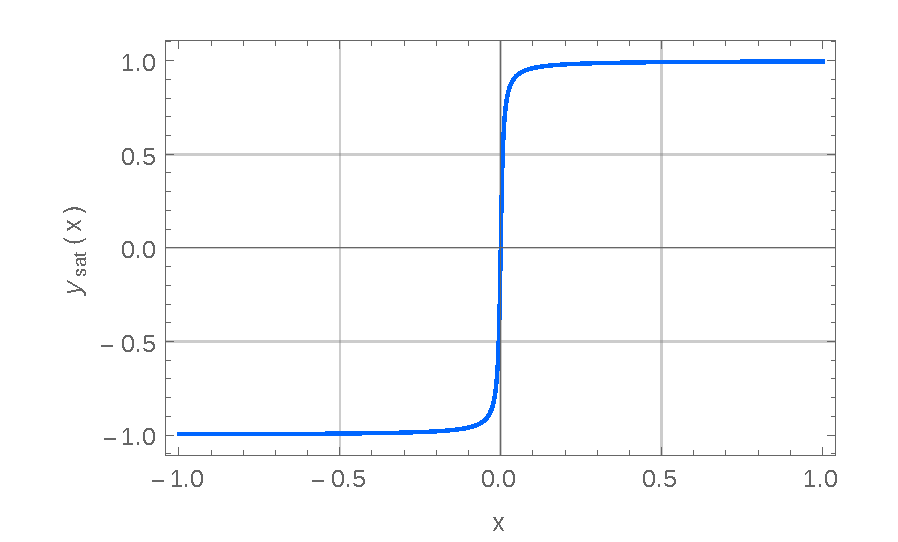
\includegraphics[scale=0.5]{Sat.pdf}
	\caption{Fun\c{c}\~ao de satura\c{c}\~ao}
	\label{Sat}
\end{figure}

Na simula\c{c}\~oes da din\^amica inversa, calculam-se os esfor\c{c}os dos atuadores necess\'arios para que o mecanismo siga exatamente a traje\'oria de refer\^encia, ignorando as condi\c{c}\~oes iniciais de velocidade que ser\~ao definidas.

\begin{itemize}
\item[A)] Simula\c{c}\~ao da trajet\'oria 1: \\

Na simula\c{c}\~ao lei de controle sup\~oe-se as seguintes condi\c{c}\~oes iniciais de velocidades:

$$\begin{cases}
\dot{q}_{1,\ttp_3,1}(0) = \dot{q}_{2,\ttp_3,1}(0) = 0 \\
\dot{q}_{1,\ttp_3,2}(0) = \dot{q}_{2,\ttp_3,2}(0) = 1 \,m/s \\
\dot{q}_{3, \llR_3}(0) = -5.871 \, rad/s \\
\dot{q}_{1,\llR_1}(0) = -4.153 \, rad/s \\
\dot{q}_{1,\llR_2}(0) = 7.089 \, rad/s \\
\dot{q}_{2,\llR_1}(0) = 4.153 \, rad/s \\
\dot{q}_{2,\llR_2}(0) = -7.089 \, rad/s \\
\end{cases}$$

Isso faz com que haja um erro de velocidade n\~ao nulo para $t=0$ e torna mais interessante a anal\'ise da din\^amica dos erros de posi\c{c}\~ao e velocidade.

Aqui seguem os gr\'aficos da trajet\'oria de refer\^encia 1 para algumas coordenadas:

\begin{figure}[H]
\centering
\begin{minipage}[b]{0.45\linewidth}
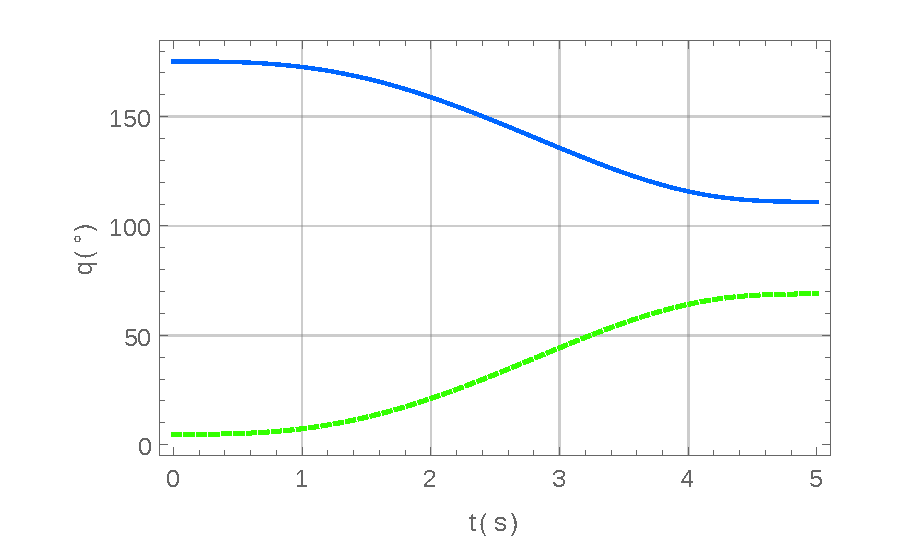
\includegraphics[scale=0.5]{AnglesA.pdf}

\includegraphics[scale=0.5]{AnglesAsub.pdf}
\label{fig:AnglesA}
\end{minipage}
\quad
\begin{minipage}[b]{0.45\linewidth}
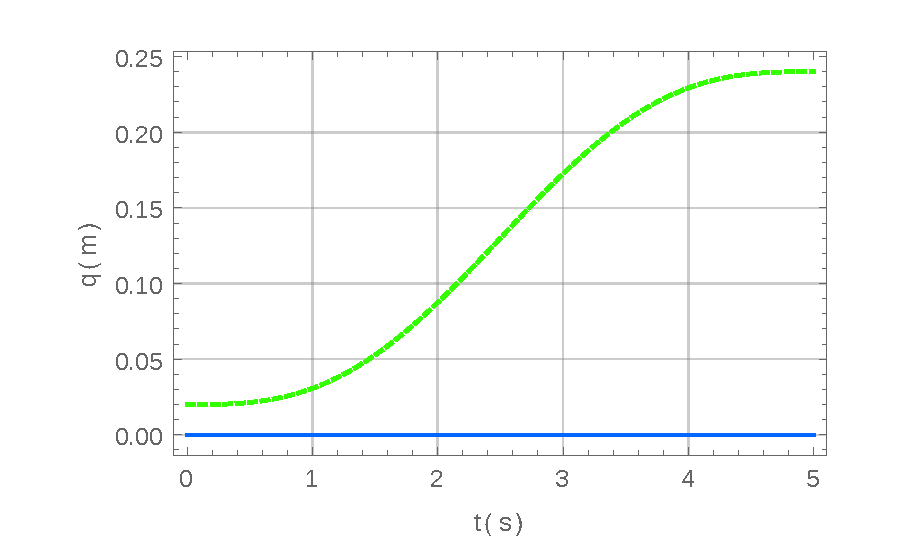
\includegraphics[scale=0.5]{XA.pdf}

\includegraphics[scale=0.5]{XAsub.pdf}
\label{fig:XA}
\end{minipage}
\caption{Trajet\'oria de refer\^encia 1}
\end{figure}

\begin{itemize}
\item[A.1)] Mecanismo balanceado \\

Simula\c{c}\~ao dos esfor\c{c}os aplicados pelos atuadores:

\begin{figure}[H]
\centering
\begin{minipage}[b]{0.45\linewidth}
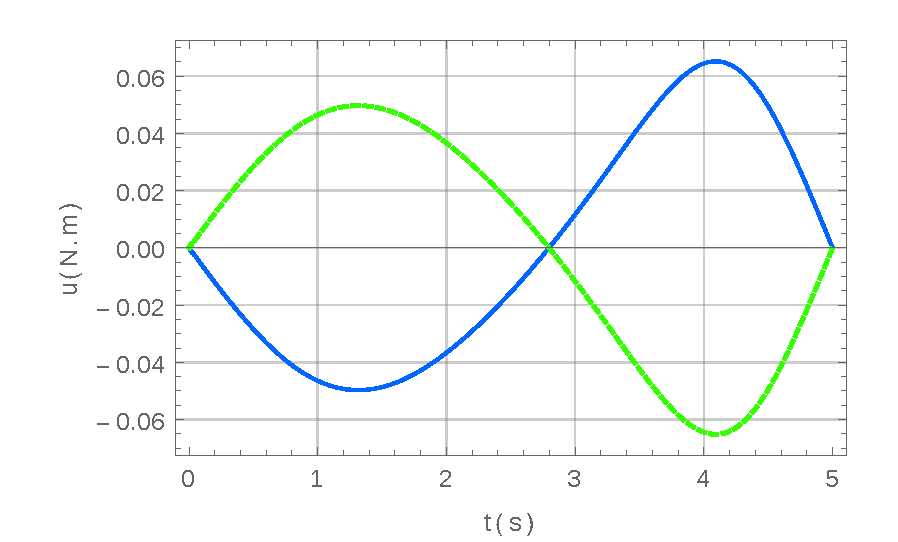
\includegraphics[scale=0.5]{InverseDynamicsA1.pdf}

\includegraphics[scale=0.5]{InverseDynamicsA1sub.pdf}
\label{fig:InverseDynamicsA1}
\caption{Inverse dynamics simulation}
\end{minipage}
\quad
\begin{minipage}[b]{0.45\linewidth}
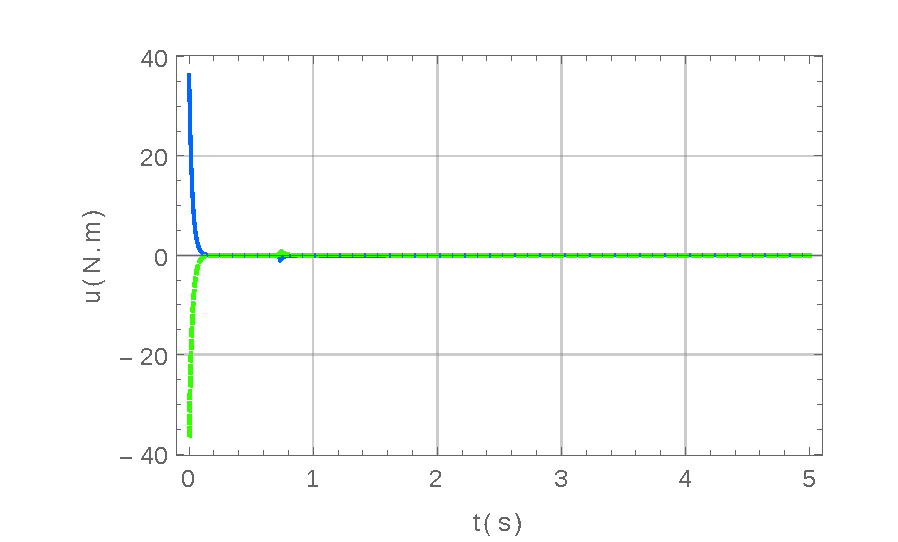
\includegraphics[scale=0.5]{ControlA1.pdf}

\includegraphics[scale=0.5]{ControlA1sub.pdf}
\label{fig:ControlA1}
\caption{Control inputs}
\end{minipage}
\quad
\begin{minipage}[b]{0.45\linewidth}
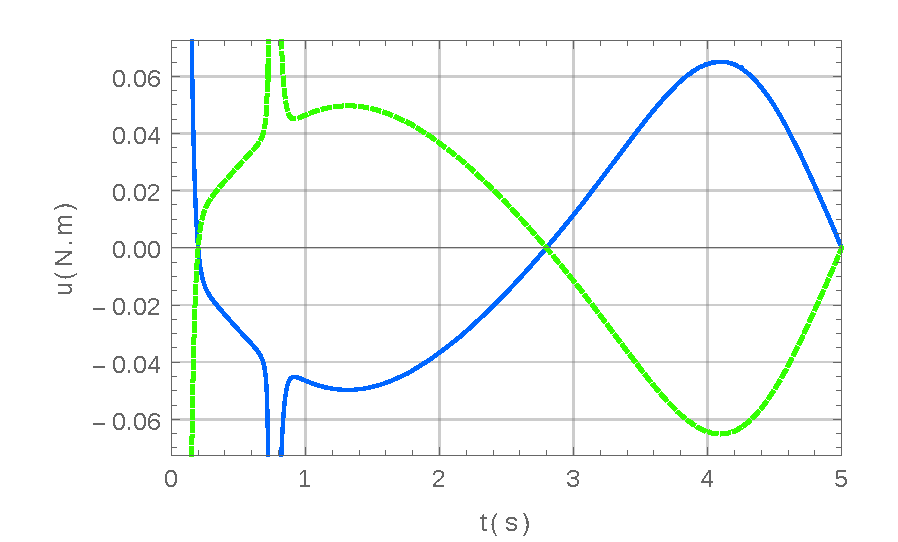
\includegraphics[scale=0.5]{ControlA1zoom.pdf}

\includegraphics[scale=0.5]{ControlA1sub.pdf}
\label{fig:ControlA1}
\caption{Control inputs (zoom)}
\end{minipage}
\end{figure}

Din\^amica do erro de controle:

\begin{figure}[H]
\centering
\subfigure[Position error norm]{%
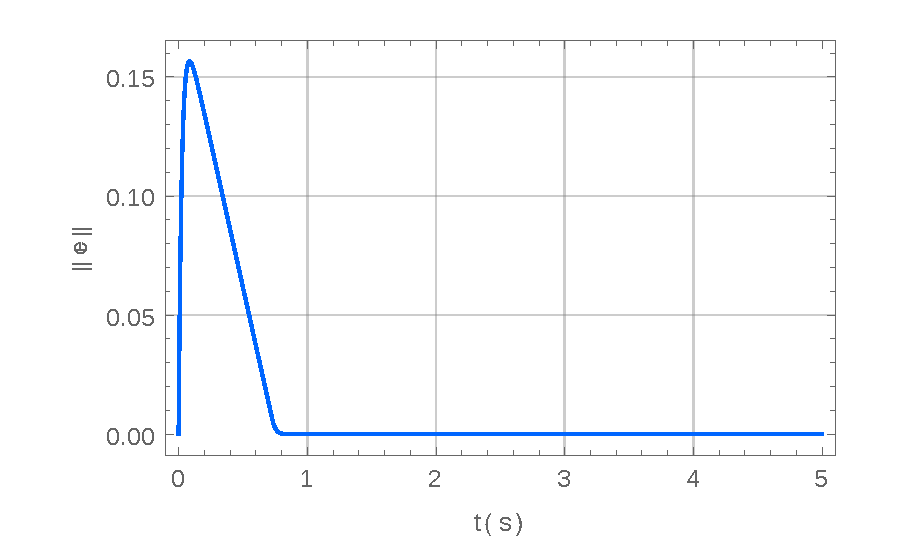
\includegraphics[scale=0.37]{PositionErrorA1.pdf}
\label{fig:PositionErrorA1}}
\quad
\subfigure[Velocity error norm]{%
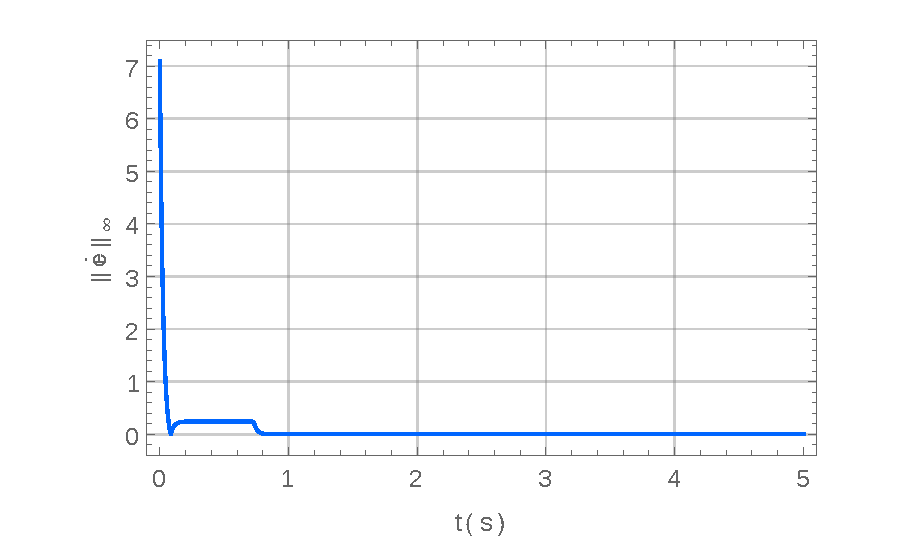
\includegraphics[scale=0.37]{VelocityErrorA1.pdf}
\label{fig:VelocityErrorA1}}
\subfigure[$\|\ms\| = \| \dot{\me} + \lambda \me \|$]{%
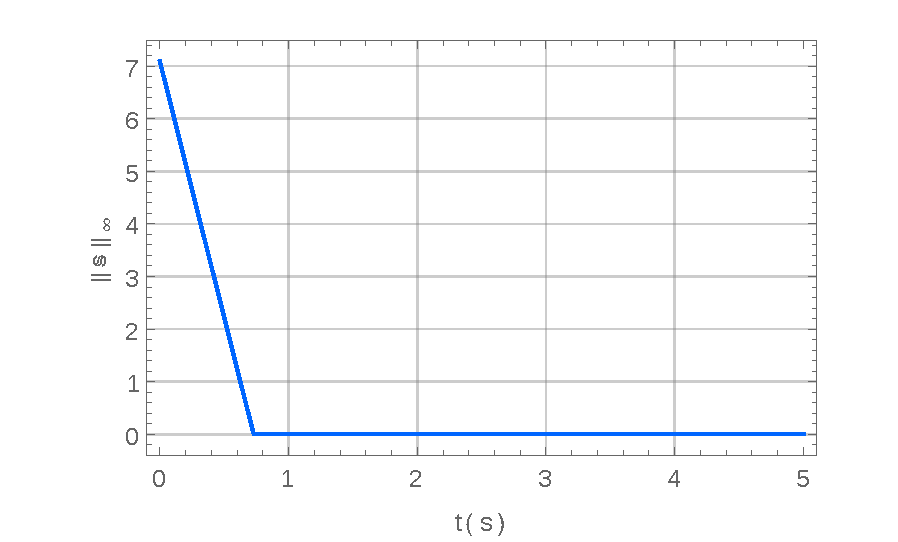
\includegraphics[scale=0.37]{sA1.pdf}
\label{fig:sA1}}
%
\caption{Error dynamics}
\label{fig:figure}
\end{figure}

\item[A.2)] Mecanismo desbalanceado \\

Simula\c{c}\~ao dos esfor\c{c}os aplicados pelos atuadores:

\begin{figure}[H]
\centering
\begin{minipage}[b]{0.45\linewidth}
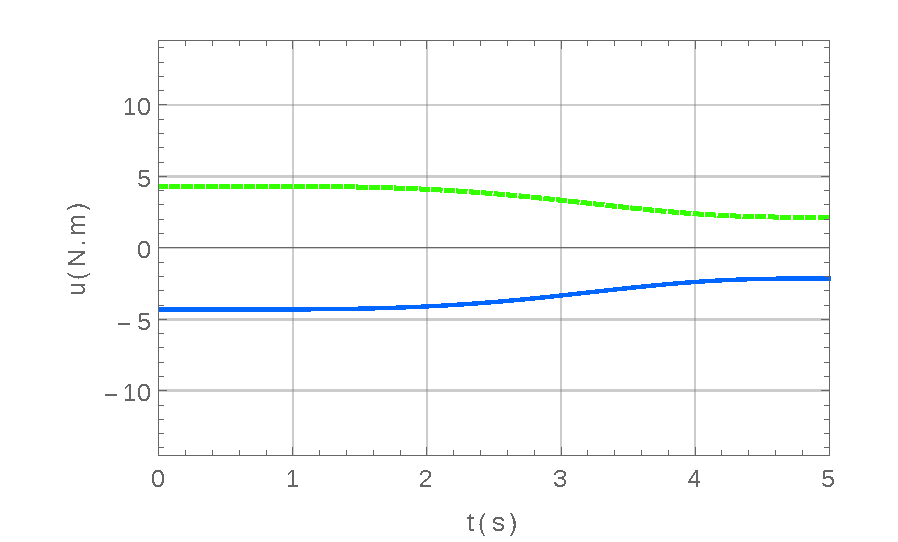
\includegraphics[scale=0.5]{InverseDynamicsA2.pdf}

\includegraphics[scale=0.5]{InverseDynamicsA1sub.pdf}
\label{fig:InverseDynamicsA2}
\caption{Inverse dynamics simulation}
\end{minipage}
\quad
\begin{minipage}[b]{0.45\linewidth}
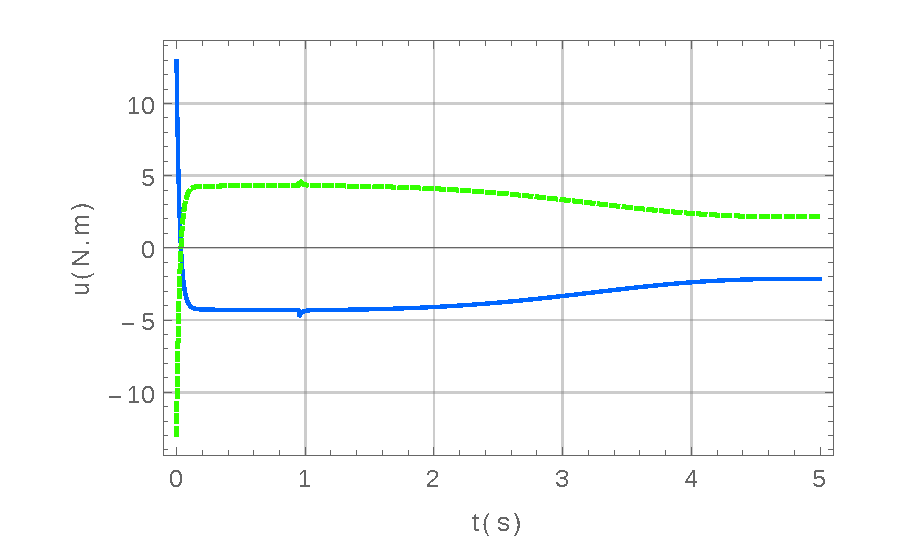
\includegraphics[scale=0.5]{ControlA2.pdf}

\includegraphics[scale=0.5]{ControlA1sub.pdf}
\label{fig:ControlA2}
\caption{Control inputs}
\end{minipage}
\end{figure}

Din\^amica do erro de controle:

\begin{figure}[H]
\centering
\subfigure[Position error norm]{%
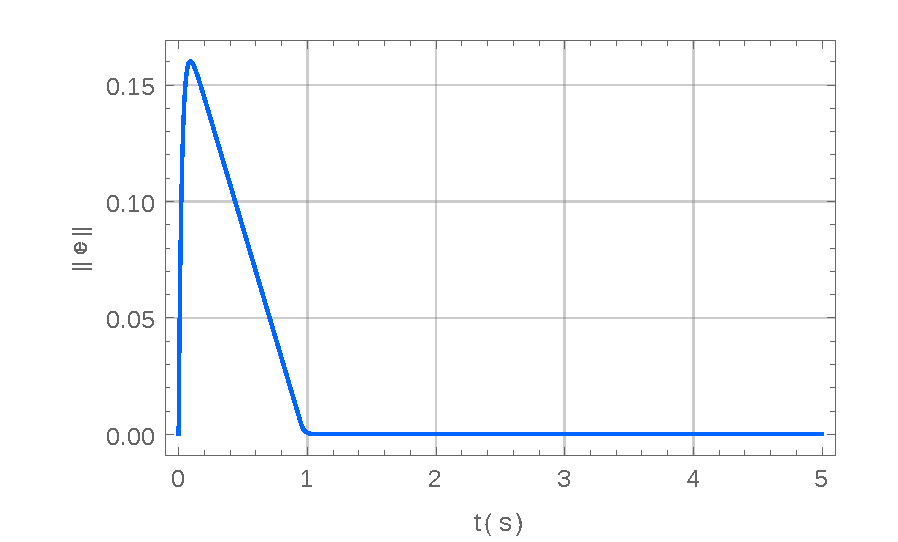
\includegraphics[scale=0.37]{PositionErrorA2.pdf}
\label{fig:PositionErrorA2}}
\quad
\subfigure[Velocity error norm]{%
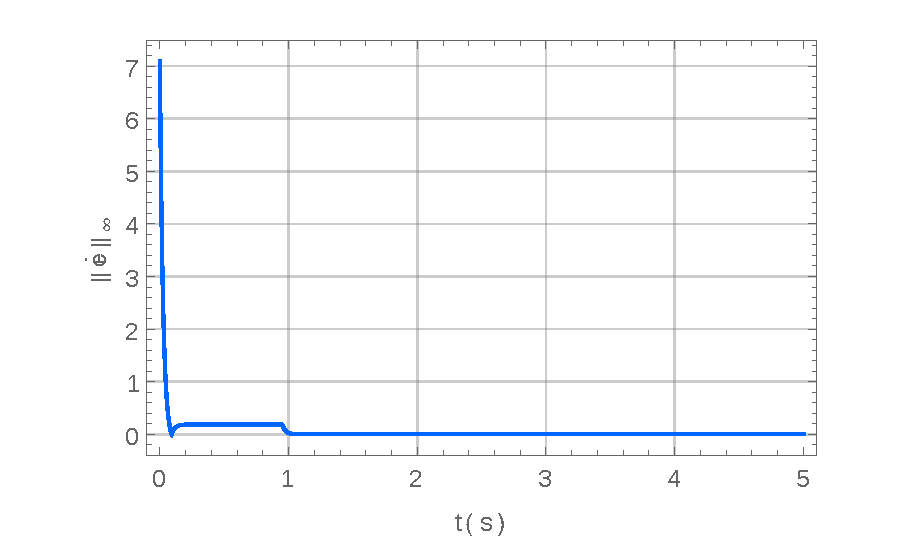
\includegraphics[scale=0.37]{VelocityErrorA2.pdf}
\label{fig:VelocityErrorA2}}
\subfigure[$\|\ms\| = \| \dot{\me} + \lambda \me \|$]{%
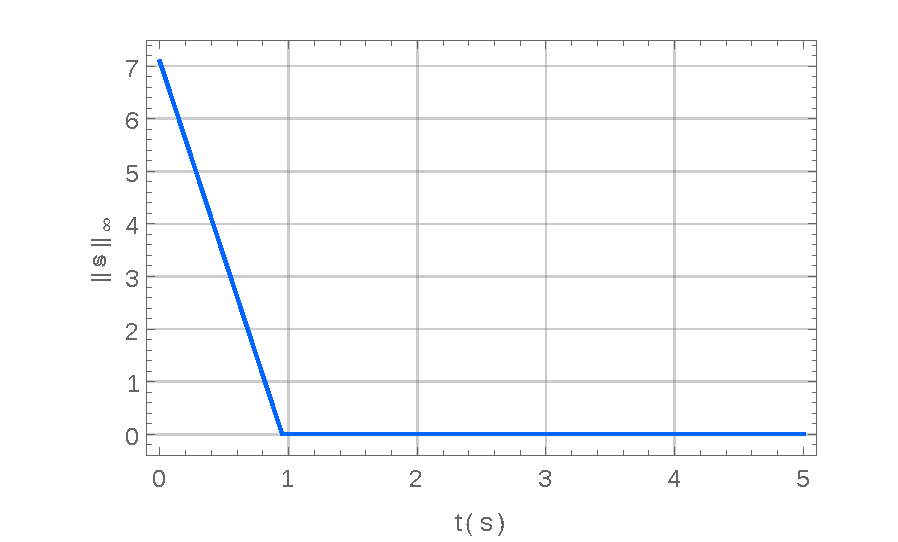
\includegraphics[scale=0.37]{sA2.pdf}
\label{fig:sA2}}
%
\caption{Error dynamics}
\label{fig:figure}
\end{figure}


\end{itemize}

Pode-se observar que, na maior parte do tempo, os esfor\c{c}os realizados pelos atuadores no caso do mecanismo desbalanceado s\~ao bem maiores do que no caso do mecanismo balanceado. Esse resultado \'e esperado, pois a trajet\'oria de refer\^encia 1 \'e um movimento lento, no qual os efeitos gravitacionais predominam ante os inerciais.


\item[B)] Simula\c{c}\~ao da trajet\'oria 2: \\

Na simula\c{c}\~ao lei de controle sup\~oe-se condi\c{c}\~oes iniciais de velocidades nulas.

Aqui seguem os gr\'aficos da trajet\'oria de refer\^encia 2 para algumas coordenadas:

\begin{figure}[ht]
\centering
\begin{minipage}[b]{0.45\linewidth}
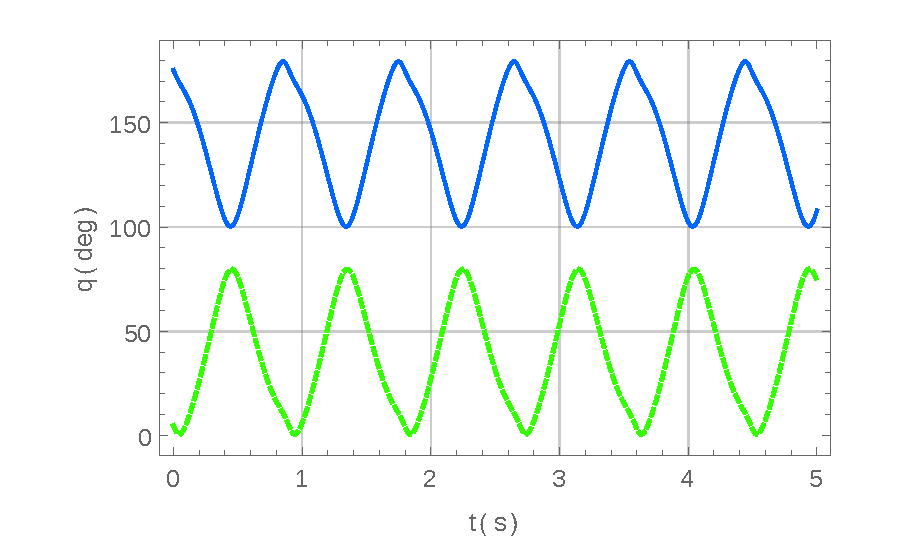
\includegraphics[scale=0.5]{AnglesB.pdf}

\includegraphics[scale=0.5]{AnglesAsub.pdf}
\label{fig:AnglesB}
\end{minipage}
\quad
\begin{minipage}[b]{0.45\linewidth}
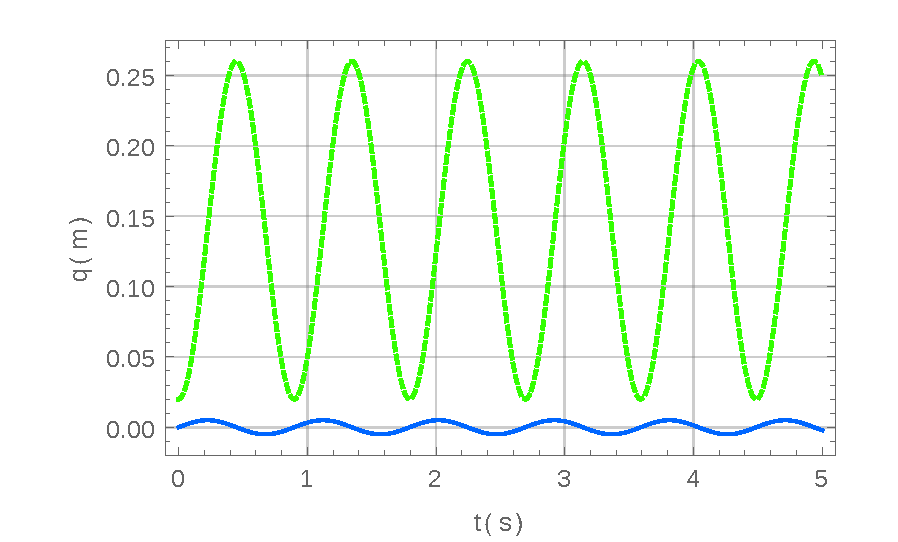
\includegraphics[scale=0.5]{XB.pdf}

\includegraphics[scale=0.5]{XAsub.pdf}
\label{fig:XB}
\end{minipage}
\caption{Trajet\'oria de refer\^encia 1}
\end{figure}

\begin{itemize}
\item[B.1)] Mecanismo balanceado \\

Simula\c{c}\~ao dos esfor\c{c}os aplicados pelos atuadores:

\begin{figure}[H]
\centering
\begin{minipage}[b]{0.45\linewidth}
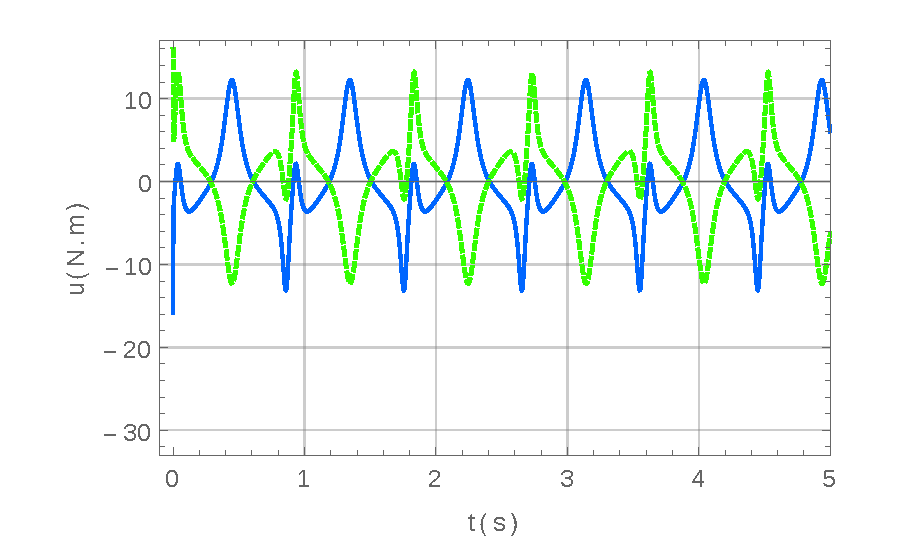
\includegraphics[scale=0.5]{InverseDynamicsB1.pdf}

\includegraphics[scale=0.5]{InverseDynamicsA1sub.pdf}
\label{fig:InverseDynamicsB1}
\caption{Inverse dynamics simulation}
\end{minipage}
\quad
\begin{minipage}[b]{0.45\linewidth}
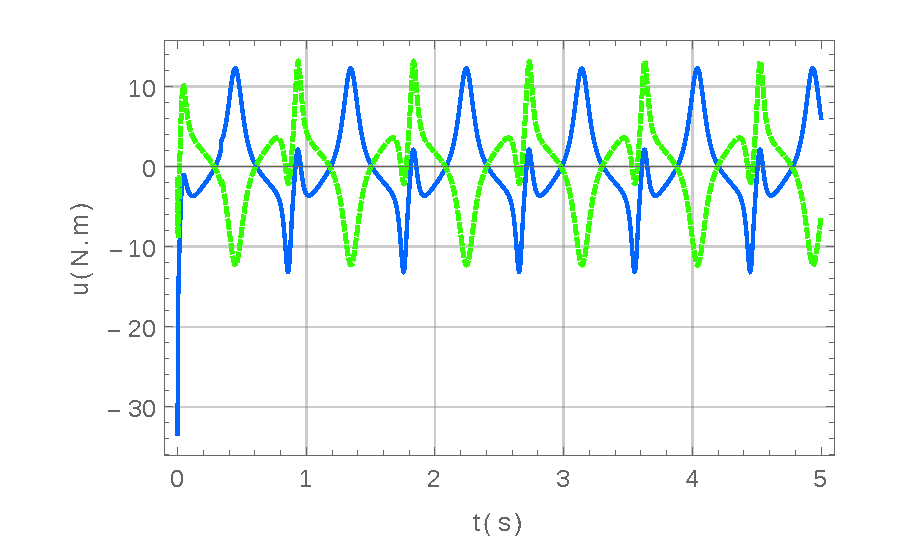
\includegraphics[scale=0.5]{ControlB1.pdf}

\includegraphics[scale=0.5]{ControlA1sub.pdf}
\label{fig:ControlB1}
\caption{Control inputs}
\end{minipage}
\end{figure}

Din\^amica do erro de controle:

\begin{figure}[H]
\centering
\subfigure[Position error norm]{%
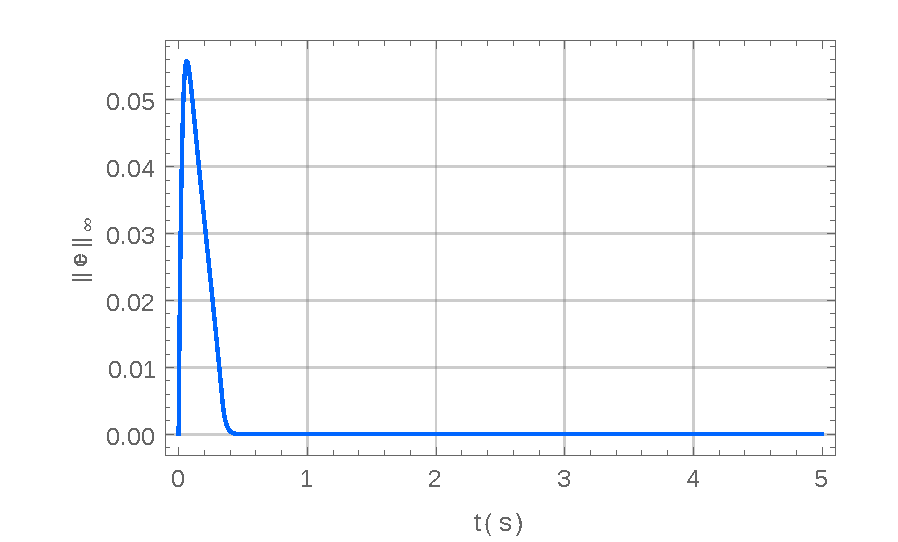
\includegraphics[scale=0.37]{PositionErrorB1.pdf}
\label{fig:PositionErrorB1}}
\quad
\subfigure[Velocity error norm]{%
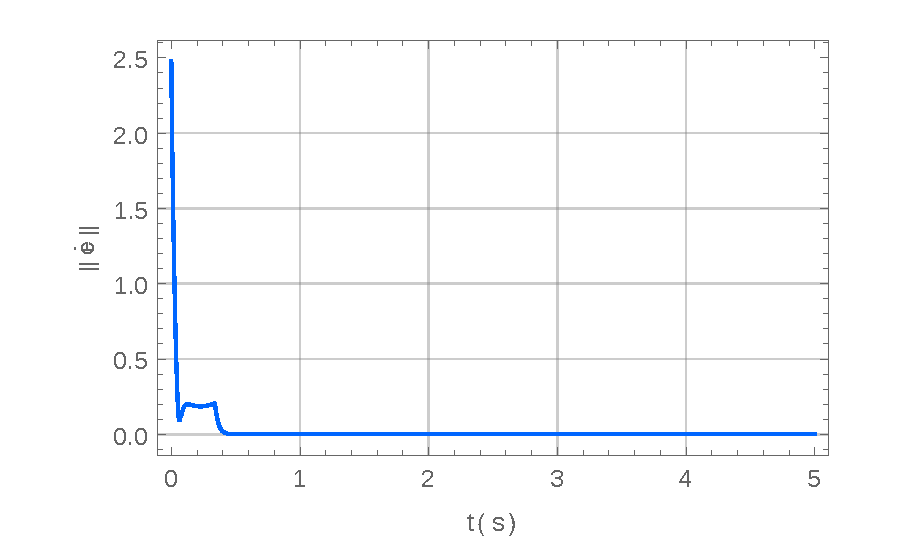
\includegraphics[scale=0.37]{VelocityErrorB1.pdf}
\label{fig:VelocityErrorB1}}
\subfigure[$\|\ms\| = \| \dot{\me} + \lambda \me \|$]{%
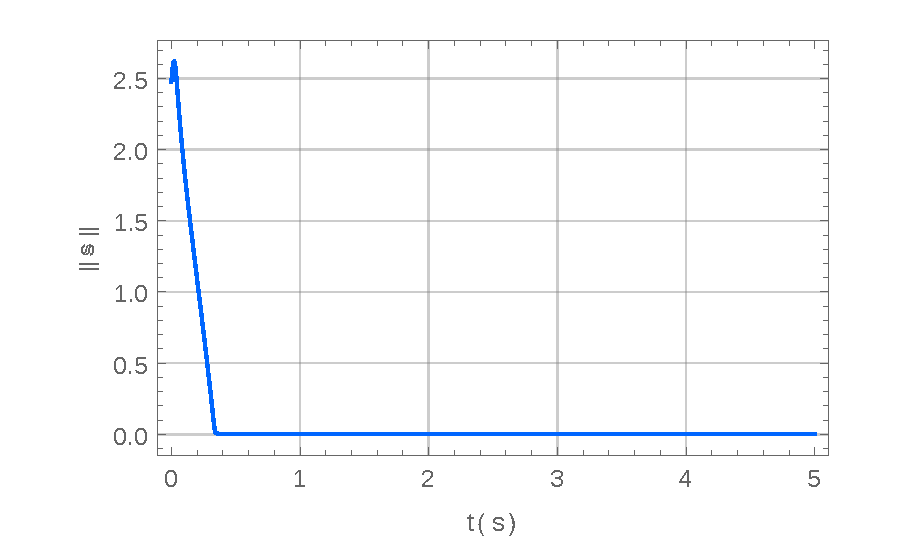
\includegraphics[scale=0.37]{sB1.pdf}
\label{fig:sA1}}
%
\caption{Error dynamics}
\label{fig:figure}
\end{figure}

\item[B.2)] Mecanismo desbalanceado \\

Simula\c{c}\~ao dos esfor\c{c}os aplicados pelos atuadores:

\begin{figure}[H]
\centering
\begin{minipage}[b]{0.45\linewidth}
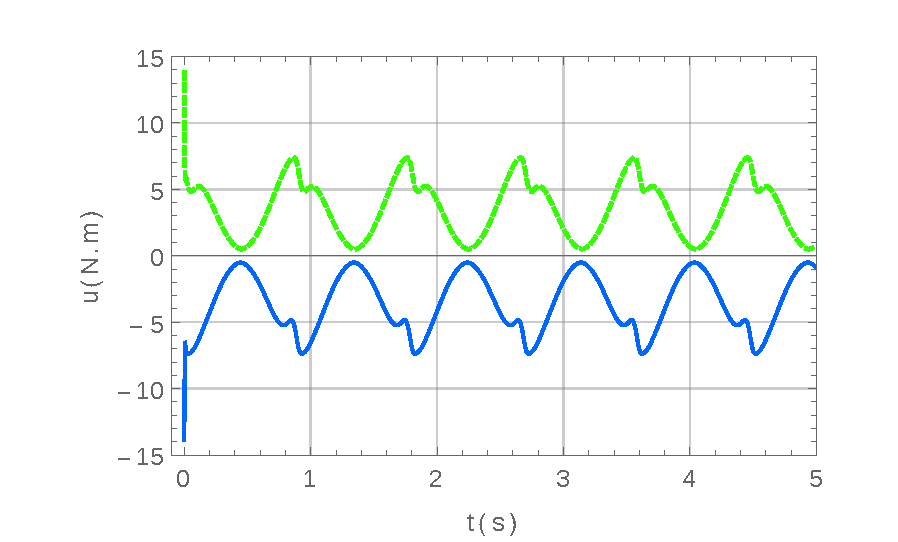
\includegraphics[scale=0.5]{InverseDynamicsB2.pdf}

\includegraphics[scale=0.5]{InverseDynamicsA1sub.pdf}
\label{fig:InverseDynamicsB2}
\caption{Inverse dynamics simulation}
\end{minipage}
\quad
\begin{minipage}[b]{0.45\linewidth}
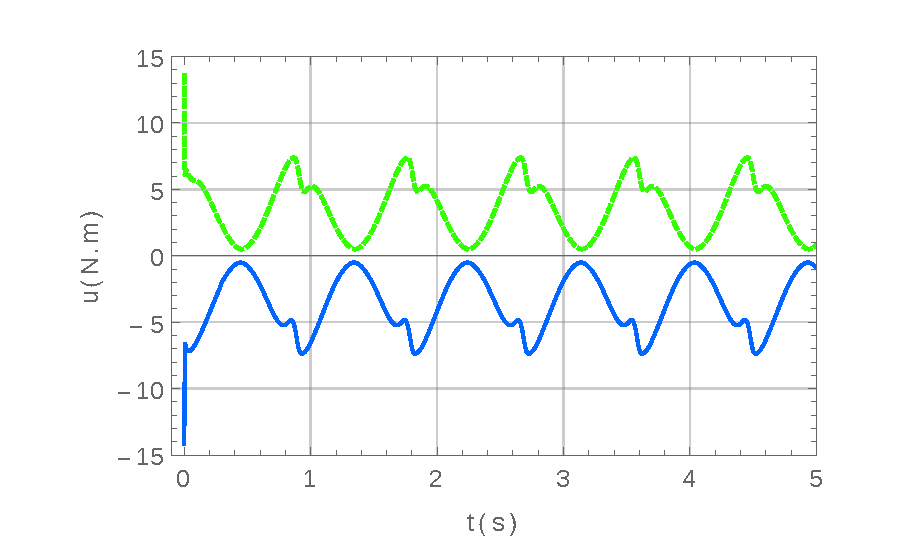
\includegraphics[scale=0.5]{ControlB2.pdf}

\includegraphics[scale=0.5]{ControlA1sub.pdf}
\label{fig:ControlB2}
\caption{Control inputs}
\end{minipage}
\end{figure}

Din\^amica do erro de controle:

\begin{figure}[H]
\centering
\subfigure[Position error norm]{%
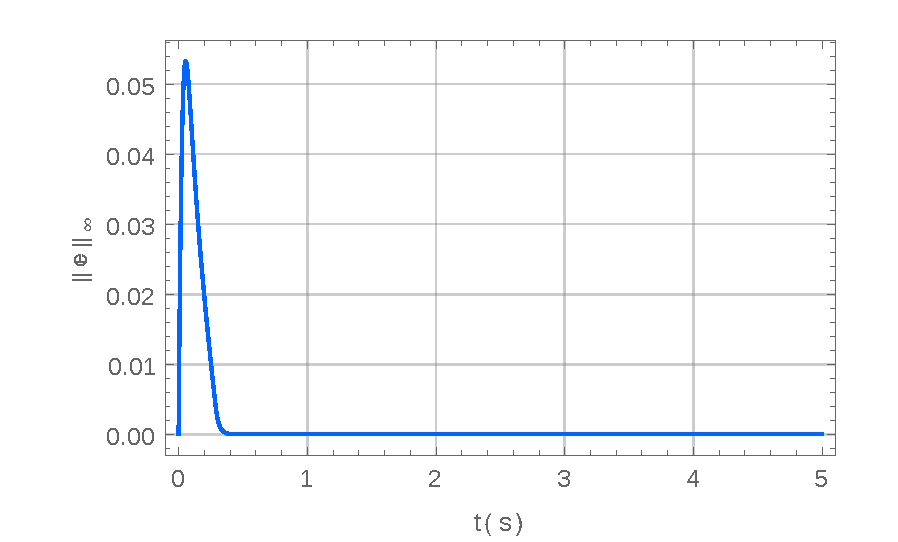
\includegraphics[scale=0.37]{PositionErrorB2.pdf}
\label{fig:PositionErrorB2}}
\quad
\subfigure[Velocity error norm]{%
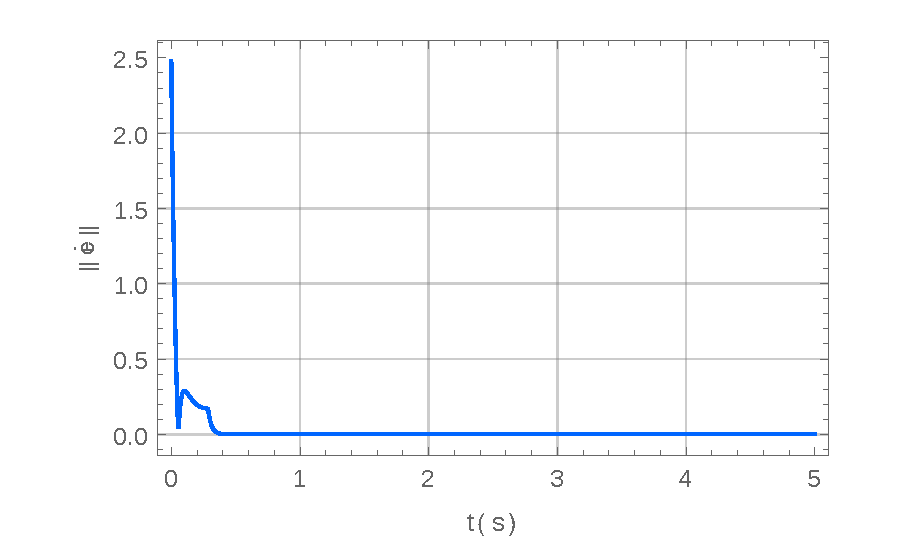
\includegraphics[scale=0.37]{VelocityErrorB2.pdf}
\label{fig:VelocityErrorB2}}
\subfigure[$\|\ms\| = \| \dot{\me} + \lambda \me \|$]{%
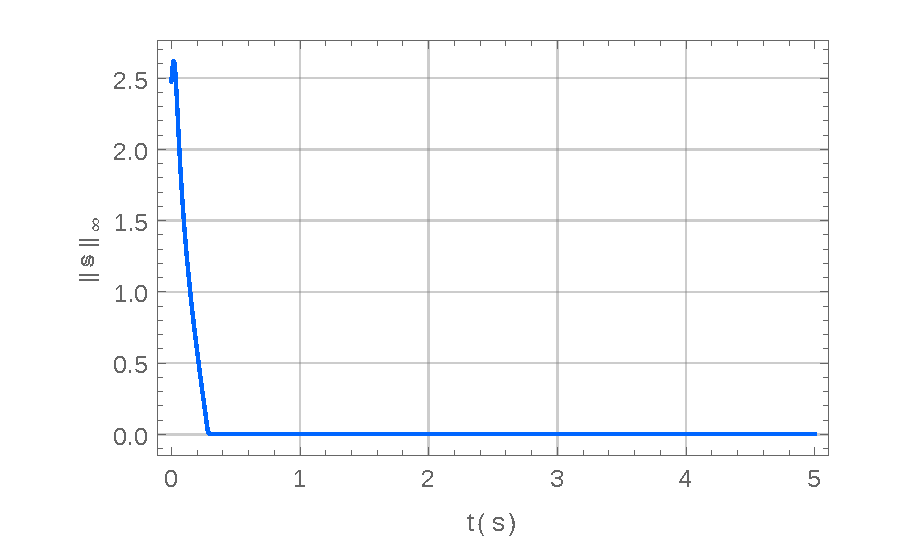
\includegraphics[scale=0.37]{sB2.pdf}
\label{fig:sB2}}
%
\caption{Error dynamics}
\label{fig:figure}
\end{figure}


\end{itemize}

Pode-se observar que, na maior parte do tempo, os esfor\c{c}os realizados pelos atuadores no caso do mecanismo desbalanceado s\~ao menores do que no caso do mecanismo balanceado. Esse resultado \'e esperado, pois a trajet\'oria de refer\^encia 2 \'e um movimento razoavelmente r\'apido, no qual os efeitos inerciais predominam ante os gravitacionais.

\end{itemize}


%--------------------CONCLUSIONS--------------------%

%\newpage

%\section{Conclusions}\label{S05}

%
% methodology
% dynamic modelling: use of redundant generalized coordinates,
%           compensation inertias (independent, modular definition)
%           successive coupling (a posteriore) without the need
%            of rewriting (a priori)
% control: sliding mode why?
% simulation results: why they are good?
% future works
%

This work dealt with the dynamic modelling and control of balanced parallel
mechanisms. The dynamic modelling process constitutes an important issue considering
the structural complexity of parallel mechanisms. 
Therefore, this book chapter described a dynamic formalism capable to deal with
redundant generalized coordinates in association with the successive coupling of additional balancing elements 
to the original system model. 
This represents {\em a posteriore} procedure because the analyst can 
successively include compensation inertias  
during the modelling
without the need of rewriting ({\em a priori} procedure) the dynamic equations.
Then, not only the compensation conditions can be derived 
but also the desired input torques for the motion control of the parallel mechanism.
This work discussed the advantages of the dynamic model,
developed in accordance with the methodology shown here, for the
sliding mode control. Finally, the simulation results have demonstrated
how effective is the presented methodology for the planar 5-bar mechanism with revolute joints. 


%--------------------ACKNOWLEDGMENTS--------------------%

%\section*{Acknowledgments}


%--------------------BIBLIOGRAPHY--------------------%

% \newpage
\phantomsection 
%

\begin{thebibliography}{99}


\bibitem{1wijk} 
V. Van der Wijk,
\newblock Shaking moment balancing of mechanisms with principal vectors and moments
\newblock {\em Front. Mech. Eng.}, 8(1): 10--16, 2013.
 
\bibitem{2arakelian}
V. H. Arakelian V. , M. R. Smith,
\newblock Design of planar 3-dof 3-RRR reactionless parallel manipulators
\newblock {\em Mechatronics}, 18: 601--606, 2008. 
 
\bibitem{3seo}
J.-T. Seo, J. H. Woo, H. Lim, J. Chung, W. K. Kim, and B.-J. Yi,
\newblock Design of an Antagonistically Counter-Balancing Parallel Mechanism
\newblock {\em IEEE/RSJ International Conference on
Intelligent Robots and Systems (IROS)}, Tokyo, November 3-7: 2882--2887, 2013. 

\bibitem{4wu}
Y. Wu, C. M. Gosselin,
\newblock Design of reactionless 3-dof and 6-dof parallel manipulators using parallelepiped mechanisms
\newblock {\em IEEE Transactions on Robotics}, 21(5): 821--833, 2005.

\bibitem{5gosselin}
C. M. Gosselin, F. Vollmer, G. C�t�, Y. Wu,
\newblock Synthesis and design of reactionless three-degree-of-freedom parallel mechanisms
\newblock {\em IEEE Transactions on Robotics and Automation}, 20(2): 191--199, 2004.

\bibitem{6wang}
J. Wang, C. M. Gosselin,
\newblock Static balancing of spatial four-degree-of-freedom parallel mechanisms
\newblock {\em Mech. Mach. Theory}, 35: 563--592, 2000.

\bibitem{7wang}
J. Wang, C. M. Gosselin,
\newblock Static balancing of spatial three-degree-of-freedom parallel mechanisms
\newblock {\em Mech. Mach. Theory}, 34: 437--452, 1999.

\bibitem{8alici}
G. Alici, B. Shirinzadeh,
\newblock Optimum Force Balancing with Mass Distribution and a Single Elastic Element for a
Five-bar Parallel Manipulator
\newblock {\em Proceedings of the IEEE International Conference on Robotics and Automation},Taipei, September 14-19: 3666--3671, 2003.

\bibitem{9alici}
G. Alici, B. Shirinzadeh,
\newblock Optimum dynamic balancing of planar parallel
manipulators based on sensitivity analysis
\newblock {\em Mech. Mach. Theory}, 41: 1520--1532, 2006.

\bibitem{10dehkordi}
M. B. Dehkordi, A. Frisoli, E. Sotgiu, M. Bergamasco,
\newblock Modelling and Experimental Evaluation of a Static Balancing Technique for
a new Horizontally Mounted 3-UPU Parallel Mechanism
\newblock {\em International Journal of Advanced Robotic Systems}, 9: 193--205, 2012.

\bibitem{11wang}
K. Wang, M. Luo, T. Mei, J. Zhao, Y. Cao,
\newblock Dynamics Analysis of a Three-DOF Planar Serial-Parallel Mechanism for Active
Dynamic Balancing with Respect to a Given Trajectory
\newblock {\em International Journal of Advanced Robotic Systems}, 10: 23--33, 2013.

\bibitem{12russo}
A. Russo, R. Sinatra, F. Xi,
\newblock Static balancing of parallel robots
\newblock {\em Mech. Mach. Theory}, 40: 191--202, 2005.

\bibitem{13agrawal}
S. K. Agrawal, A. Fattah,
\newblock Gravity-balancing of spatial robotic manipulators
\newblock {\em Mech. Mach. Theory}, 39: 1331--1344, 2004.

\bibitem{14briot}
S. Briot, V. Arakelian, J.-P. Le Baron,
\newblock Shaking force minimization of high-speed robots via centre of mass
acceleration control
\newblock {\em Mech. Mach. Theory}, 57: 1--12, 2012.

\bibitem{15coelho}
T. A. H. Coelho, L. Yong, V. F. A. Alves,
\newblock Decoupling of dynamic equations by means of
adaptive balancing of 2-dof open-loop mechanisms
\newblock {\em Mech. Mach. Theory}, 39: 871--881, 2004.

\bibitem{16moradi}
M. Moradi, A. Nikoobin, S. Azadi,
\newblock Adaptive Decoupling for Open Chain Planar Robots
\newblock {\em Transaction B: Mechanical Engineering}, 17(5): 376--386, 2010.

\bibitem{17arakelian}
V. Arakelian, S. Sargsyan,
\newblock On the design of serial manipulators with decoupled dynamics
\newblock {\em Mechatronics}, 22(6): 904--909, 2012.

\bibitem{18tsai}
J. Chen, D.Z. Chen, L.W. Tsai,
\newblock A Systematic Methodology for the Dynamic Analysis of Articulated Gear-Mechanisms,
\newblock 1990.

\bibitem{19kane}
T. R. Kane, D. A. Levinson,
\newblock {\em {Dynamics, Theory and Applications}}.
\newblock McGraw-Hill series in mechanical engineering. McGraw Hill, 1985.

\bibitem{20altuzarra}
O. Altuzarra, P. M. Eggers, F. J. Campa, C. Roldan-Paraponiaris, C. Pinto, 
\newblock Dynamic Modelling of Lower-Mobility Parallel Manipulators Using the Boltzmann-Hamel Equations
\newblock {\em Mechanisms, Transmissions and Applications}, 31: 157--165, 2015.

\bibitem{21orsino}
R. M. M. Orsino, T. A. H. Coelho, C. P. Pesce, 
\newblock Analytical mechanics approaches in the dynamic modelling of Delta mechanism
\newblock {\em Robotica}, 33(4): 953--973, 2015.

\bibitem{22orsino}
R. M. M. Orsino, A. G. Coutinho, T. A. H. Coelho,
\newblock Dynamic modelling and control of balanced parallel mechanisms.
\newblock Book chapter of {\em Dynamic Balancing of Mechanisms and Synthesizing of Parallel Robots}, Springer, 2016 (in press).

\bibitem{23orsino}
R. M. M. Orsino, T. A. H. Coelho (2015).
\newblock A contribution on the modular modelling of multibody systems.
\newblock Manuscript submitted for publication

\end{thebibliography}


%\end{document}


% \end{multicols}


\end{document}

